\index{general}{MMS} 
\index{general}{Method of Manufactured Solutions}
\begin{flushright} {\tiny {\color{gray} mms.tex}} \end{flushright}
%~~~~~~~~~~~~~~~~~~~~~~~~~~~~~~~~~~~~~~~~~~~~~~~~~~~~~~~~~~~~~~~~~~~~~~~~~~~~~~~~~~~~~~~~~~~~~~~~~~

The method of manufactured solutions is a relatively simple way of carrying out
code verification. In essence, one postulates a solution for the PDE at hand (as
well as the proper boundary conditions), inserts it in the PDE and computes the 
corresponding source term. 
The same source term and boundary conditions will then be used in a numerical 
simulation so that the computed solution can be compared with the (postulated)
true analytical solution. 

Examples of this approach are to be found in \cite{dohu03,busa13,bodg06,polp14,polp14b,lopp14,blmp16}.

%-----------------------------------------------------------------------------
\subsubsection{Analytical benchmark I \label{mms1} - "DH"}

Taken from \cite{dohu03}. We consider a two-dimensional problem 
in the square domain $\Omega=[0,1]\times[0,1]$, which possesses a closed-form analytical 
solution. The problem consists of determining the velocity field ${\vec \upnu} = (u,v)$ 
and the pressure $p$ such that 
\begin{eqnarray}
\eta \Delta {\vec \upnu} - {\vec \nabla} p + {\vec b} &=& \vec 0 \quad\quad {\rm in} \; \Omega\\
\vec{\nabla} \cdot \vec{v} &=& 0 \quad\quad {\rm in} \; \Omega\\
\vec{v}&=&\vec{0} \quad\quad {\rm on} \; \Gamma_D
\end{eqnarray}
where the fluid viscosity is taken as $\eta=1$.
The components of the body force $\vec{b}$ are prescribed as 
\begin{eqnarray}
b_x &=& (12 - 24y) x^4 + (-24 + 48y) x^3 + (-48y + 72y^2 - 48 y^3 + 12) x^2 \nonumber\\
    && + (-2 + 24y -72y^2+48y^3)x + 1-4y + 12y^2-8y^3 \nonumber\\ 
b_y &=& (8 - 48y + 48 y^2) x^3 + (-12 + 72y - 72y^2) x^2  \nonumber\\
    && + (4 - 24y + 48y^2 - 48y^3 + 24y^4) x - 12y^2 + 24y^3 - 12y^4  \nonumber
\end{eqnarray}
With this prescribed body force, the exact solution is 
\begin{eqnarray}
u(x,y) &=& x^2(1- x)^2 (2y - 6y^2 + 4y^3)  \nonumber\\
v(x,y) &=& -y^2 (1 - y)^2 (2x - 6x^2 + 4x^3) \nonumber\\
p(x,y) &=& x(1 -x)- 1/6 \nonumber 
\end{eqnarray}
Note that the pressure obeys $\int_{\Omega} p \; dV = 0$.
One can turn to the spatial derivatives of the fields:
\begin{eqnarray}
\dot{\varepsilon}_{xx}=\frac{\partial u}{\partial x} &=&  (2x -6x^2 +4 x^3 ) (2y - 6y^2 + 4y^3)  \\
\dot{\varepsilon}_{yy}=\frac{\partial v}{\partial y} &=&  - (2x -6x^2 +4 x^3 ) (2y - 6y^2 + 4y^3)  \\
\dot{\varepsilon}_{xy}=\frac{1}{2}\left(\frac{\partial u}{\partial y}+\frac{\partial v}{\partial x}\right) 
&=&=\frac{1}{2}\left( x^2(1- x)^2 ( 2-12y+12y^2  ) -y^2 (1-y)^2 (2-12x+12x^2) \right)
\end{eqnarray}
with of course  ${\vec \nabla} \cdot {\vec \upnu} = 0$ and 
\begin{eqnarray}
\frac{\partial p}{\partial x} &=& 1-2x  \\
\frac{\partial p}{\partial y} &=& 0
\end{eqnarray}

The velocity and pressure fields look like:

\begin{center}
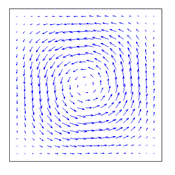
\includegraphics[height=4cm]{images/mms/Ex1_Q2Q1_velo.png}
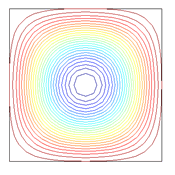
\includegraphics[height=4cm]{images/mms/Ex1_Q2Q1_streamlines.png}
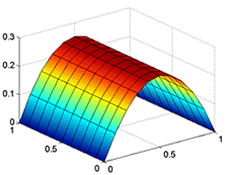
\includegraphics[height=4cm]{images/mms/Ex1_Q2Q1_pres.png}\\
{\small http://ww2.lacan.upc.edu/huerta/exercises/Incompressible/Incompressible\_Ex1.htm}
\end{center}

As shown in \cite{dohu03}, If the LBB condition is not satisfied, spurious oscillations spoil the pressure approximation. 
Figures below show results obtained with a mesh of 20x20 $Q_1\times P_0$ (left) and $P_1\times P_1$ (right) elements:
\begin{center}
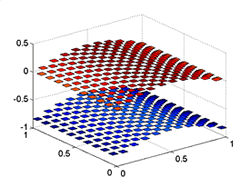
\includegraphics[height=5cm]{images/mms/Ex1_Q1P0_pres.png}
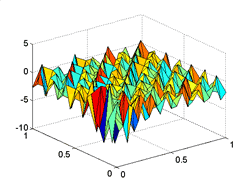
\includegraphics[height=5cm]{images/mms/Ex1_P1P1_pres.png}]]
{\small http://ww2.lacan.upc.edu/huerta/exercises/Incompressible/Incompressible\_Ex1.htm}
\end{center}

Taking into account that the proposed problem has got analytical solution, it is easy to analyze convergence of the different pairs of elements:
\begin{center}
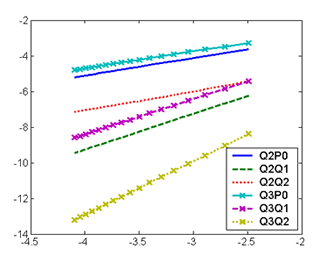
\includegraphics[height=7cm]{images/mms/Ex1_conv_qua.png}\\
{\small http://ww2.lacan.upc.edu/huerta/exercises/Incompressible/Incompressible\_Ex1.htm}
\end{center}

One can also compute the stress components:
\begin{eqnarray}
\sigma_{xx} &=&  2x^2(2x - 2)(4y^3 - 6y^2 + 2y) + 4x(-x + 1)^2*(4y^3 - 6y^2 + 2y) - x(-x + 1) + 1/6 \\
\sigma_{xy} &=&  x^2(-x + 1)^2*(12y^2 - 12y + 2) - y^2(-y + 1)^2*(12x^2 - 12x + 2) \\
\sigma_{yy} &=&  -x(-x + 1) - 2y^2(2y - 2)(4x^3 - 6x^2 + 2x) - 4y(-y + 1)^2(4x^3 - 6x^2 + 2x) + 1/6
\end{eqnarray}

All the necessary functions to do this benchmark are in {\tt mms/dh.py}:
\lstinputlisting[language=python]{mms/dh.py}

This benchmark is implemented in \aspect{} \cite{aspectmanual} and in \stone 1 and many more.

We have
\[
\int_0^1 \int_0^1 u^2 dxdy=
\int_0^1 \int_0^1 ( x^2(1- x)^2 (2y - 6y^2 + 4y^3)  )^2 dx dy = \frac{1}{33075}
\]
\[
\int_0^1 \int_0^1 v^2 dxdy=
\int_0^1 \int_0^1 ( -y^2 (1 - y)^2 (2x - 6x^2 + 4x^3) )^2 dx dy = \frac{1}{33075}
\]
so the root mean square velocity is  
\[
v_{rms} = \sqrt{ \frac{1}{L_x L_y}  \int_0^1 \int_0^1 (u^2+v^2) dx dy } \simeq 0.00777615791
\]



%-----------------------------------------------------------------------------
\subsubsection{Analytical benchmark II \label{ss:mms2} - "DB2D"}

Taken from Dohrmann \& Bochev (2004,2006) \cite{dobo04,bodg06}. 
This benchmark is also used in Worthen \etal \cite{wosp14} and Lamichhane \etal \cite{lami17}.
It is for a unit square with $\nu=\eta/\rho=1$ and the smooth exact solution is
\begin{eqnarray}
u(x,y) &=& x+x^2 - 2xy+x^3 - 3xy^2 + x^2y \\
v(x,y) &=& -y-2xy+y^2 -3x^2y + y^3 - xy^2 \\
p(x,y) &=& xy+x+y+x^3y^2 - 4/3
\end{eqnarray}
Note that the pressure field is such that $\int_{\Omega} p \; dV = 0$.
The gradient components of the velocity and pressure fields are given by:
\begin{eqnarray}
\frac{\partial u}{\partial x} &=& 3x^2+2x(y+1)-3y^2-2y+1   \\
\frac{\partial u}{\partial y} &=& x(x-6y-2)\\
\frac{\partial v}{\partial x} &=& -y(6x+y+2)\\
\frac{\partial v}{\partial y} &=& -3x^2-2x(y+1)+3y^2+2y-1 \\
\frac{\partial p}{\partial x} &=& 3x^2y^2 + y +1 \\ 
\frac{\partial p}{\partial y} &=& 2x^3y+x+1 
\end{eqnarray}
so that the strain rate tensor components are 
\begin{eqnarray}
\dot{\varepsilon}_{xx} &=&  3x^2+2x(y+1)-3y^2-2y+1 \\
\dot{\varepsilon}_{yy} &=& -3x^2-2x(y+1)+3y^2+2y-1 \\
\dot{\varepsilon}_{xy} &=&  \frac{1}{2} [x(x-6y-2) -y(6x+y+2) ] \\
&=& \frac{1}{2}( x^2 -y^2 -12xy -2x -2y)
\end{eqnarray}
We have
\begin{eqnarray}
\frac{\partial \dot{\varepsilon}_{xx}}{\partial x} &=& 2(3x+y+1) \\
\frac{\partial \dot{\varepsilon}_{xy}}{\partial y} &=& -6x-y-1  \\
\frac{\partial \dot{\varepsilon}_{xy}}{\partial x} &=&  -6y+x-1 \\  
\frac{\partial \dot{\varepsilon}_{yy}}{\partial y} &=& 2(3y-x+1) 
\end{eqnarray}
so that the corresponding body force is given by:
\begin{eqnarray}
b_x 
&=& \frac{\partial p}{\partial x}  
-2\frac{\partial \dot{\varepsilon}_{xx}}{\partial x} -  2\frac{\partial \dot{\varepsilon}_{xy}}{\partial y} \nn\\
&=& 3x^2y^2 + y +1  - 4(3x+y+1) - 2(-6x-y-1) \nn\\
&=& 3x^2y^2 -y-1   \\
b_y 
&=& \frac{\partial p}{\partial y} 
-2 \frac{\partial \dot{\varepsilon}_{xy}}{\partial x} - 2\frac{\partial \dot{\varepsilon}_{yy}}{\partial y}  \nn\\
&=& 2x^3y+x+1  -2(-6y+x-1) - 4(3y-x+1) \nn\\
&=& 2x^3y+3x-1 
\end{eqnarray}

Finally we have
\[
\int_0^1 \int_0^1 u^2 dxdy=
\int_0^1 \int_0^1 ( x+x^2 - 2xy+x^3 - 3xy^2 + x^2y  )^2 dx dy = \frac{401}{504} 
\]
\[
\int_0^1 \int_0^1 v^2 dxdy=
\int_0^1 \int_0^1 (-y-2xy+y^2 -3x^2y + y^3 - xy^2  )^2 dx dy = \frac{5911}{2520}
\]
so the root mean square velocity is
\[
v_{rms} = \sqrt{ \frac{1}{L_x L_y}  \int_0^1 \int_0^1 (u^2+v^2) dx dy }  
= \sqrt{\frac{401\cdot 5 + 5911}{2520}}\simeq 1.77236278... 
\]





%-----------------------------------------------------------------------------
\subsubsection{Analytical benchmark III \label{mms3} - "DB3D"}

This benchmark begins by postulating a polynomial solution 
to the 3D Stokes equation \cite{dobo04}:
\begin{equation}
\vec{\upnu}
=
\left(
\begin{array}{c}
x+x^2+xy+x^3y \\
y + xy + y^2 + x^2 y^2\\
-2z - 3xz - 3yz - 5x^2 yz
\end{array}
\right)
\label{eqbur}
\end{equation}
and
\begin{equation}
p = xyz + x^3 y^3z - 5/32
\end{equation}
While it is then trivial to verify that this velocity field is divergence-free (see here under),  
the corresponding body force of the Stokes equation can be computed by  
inserting this solution into the momentum equation with a given viscosity $\eta(x,y,z)$
(constant or position/velocity/strain rate dependent). 
The domain is a unit cube and velocity boundary conditions 
simply use Eq. (\ref{eqbur}). 
Note that the pressure fulfils 
\[
\int_\Omega p(x,y,z) dV = 0.  
\]
Following \cite{busa13}, the viscosity
is given by the smoothly varying function
\begin{equation}
\eta(x,y,z) = exp(1 - \beta(x(1 - x) + y(1 - y) + z(1 - z)))
\end{equation}
Choosing $\beta=0$ yields a constant velocity $\eta=e^1$ (and greatly simplifies the right-hand side).
One can easily show that the ratio of viscosities $\eta^\star$
in the system follows $\eta^\star=\exp(-3\beta/4)$ so that choosing $\beta=10$ yields
$\eta^\star\simeq 1808$ and $\beta=20$ yields $\eta^\star\simeq 3.269\times10^6$.

The exact form of the rhs is carried out in Stone \ref{f17}.

Let us now compute the root mean square velocity:
\begin{eqnarray}
\int_\Omega u^2 dx dy dz &=& \int_{0}^{+1}\int_{0}^{+1}\int_{0}^{+1} (x+x^2+xy+x^3y )^2 dx dy dz = 2867/1260 \\
\int_\Omega v^2 dx dy dz &=& \int_{0}^{+1}\int_{0}^{+1}\int_{0}^{+1} (y + xy + y^2 + x^2 y^2 )^2 dx dy dz = 3947/1800   \\
\int_\Omega w^2 dx dy dz &=& \int_{0}^{+1}\int_{0}^{+1}\int_{0}^{+1} (-2z - 3xz - 3yz - 5x^2 yz )^2 dx dy dz = 463/36   
\end{eqnarray}
then
\[
\upnu_{rms}=\sqrt{ 2867/1260 + 3947/1800 + 463/36  } \simeq 4.1628459
\]



%-----------------------------------------------------------------------------
\subsubsection{Analytical benchmark IV \label{mms4} - "Bercovier \& Engelman"}

From \cite{been79}. The two-dimensional domain is a unit square. The body forces are:
\begin{eqnarray}
f_x &=& 128[ x^2(x-1)^2 12 (2y-1) + 2 (y-1)(2y-1)y(12x^2-12x+2)  ] \nn\\
f_y &=& 128[ y^2(y-1)^2 12 (2x-1) + 2 (x-1)(2x-1)y(12y^2-12y+2)  ] \nn\\
\end{eqnarray}
The solution is
\begin{eqnarray}
u &=& -256x^2(x-1)^2y(y-1)(2y-1) \nn\\
v &=&  256y^2(y-1)^2x(x-1)(2x-1) \nn\\
p &=& 0 
%p &=& (x-1/2)(y-1/2) 
\end{eqnarray}

\begin{eqnarray}
du/dx &=& 512 (1 - 2x) (-1+x) x(-1+y) y(-1+2y) \\ 
du/dy &=& -256 (-1 + x)^2 x^2 (1 - 6 y + 6 y^2) \\ 
dv/dx &=&  256y^2(y-1)^2x(x-1)(2x-1) \\ 
dv/dy &=& -512 (-1 + x) x (1 - 2 x) (-1 + y) y (-1 + 2 y) \\
\end{eqnarray}

and we can easily verify that $\vec\nabla\cdot\vec\upnu=du/dx+dv/dy=0$.

CHECK RHS !

Another choice with a non-zero pressure:
\begin{eqnarray}
f_x &=& 128[ x^2(x-1)^2 12 (2y-1) + 2 (y-1)(2y-1)y(12x^2-12x+2)  ] + y - 1/2 \nn\\
f_y &=& 128[ y^2(y-1)^2 12 (2x-1) + 2 (x-1)(2x-1)y(12y^2-12y+2)  ] + x - 1/2 \nn\\
\end{eqnarray}
The solution is
\begin{eqnarray}
u &=& -256x^2(x-1)^2y(y-1)(2y-1) \nn\\
v &=&  256y^2(y-1)^2x(x-1)(2x-1) \nn\\
p &=& (x-1/2)(y-1/2) 
\end{eqnarray}


%-----------------------------------------------------------------------------
\subsubsection{Analytical benchmark V \label{mms5} - "VJ1"}

This is taken from Appendix D1 of \cite{john16}.

The domain $\Omega$ is a unit square. We consider the stream function
\[
\phi(x,y)=1000x^2(1-x)^4y^3(1-y)^2
\]
The velocity field is defined by
\begin{eqnarray}
u(x,y) &=&  \partial_y \phi = 1000(x^2(1-x)^4 y^2 (1-y)(3-5y)  ) \\
v(x,y) &=& -\partial_x \phi = 1000(-2x(1-x)^3(1-3x)y^3(1-y)^2)
\end{eqnarray}
and it is easy to verify that $\vec\nabla\cdot\vec v=0$.

The pressure is given by:
\[
p(x,y)=\pi^2( xy^3\cos(2\pi x^2y) - x^2y \sin(2\pi xy)) + \frac{1}{8}
\]

\begin{center}
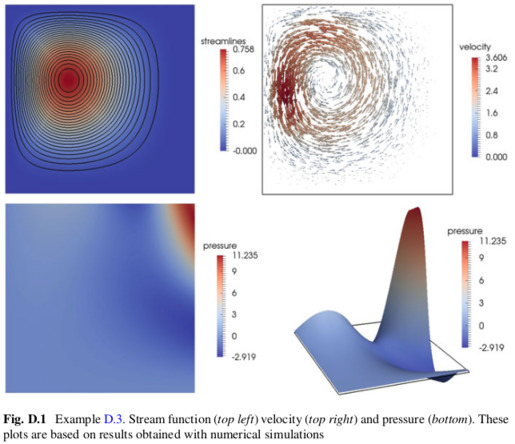
\includegraphics[width=8cm]{images/mms/mms5}\\
Taken from \cite{john16}.
\end{center}

\bscthesis \index{general}{BSc Thesis}

%-----------------------------------------------------------------------------
\subsubsection{Analytical benchmark VI \label{mms6} - "Ilinca \& Pelletier"}
\index{general}{Poiseuille flow} \index{general}{Shear Heating}

This is taken from \cite{ilpe07}.

Let us consider the Poiseuille flow of a Newtonian fluid. The channel has 
isothermal flat walls located at $y=\pm h$. The velocity distribution is parabolic:
\[
u = u_0 \left(1-\frac{y^2}{h^2} \right) 
\quad\quad\quad
v=0
\]
where $u_0$ is the maximum velocity. The (steady state) temperature field is the solution of
the advection-diffusion equation:
\[
\rho C_p \vec v \cdot \vec\nabla T
= k \Delta T + \Phi
\]
where $\Phi$ is the dissipation function given by
\[
\Phi
=\eta \left[  
2\left(\frac{\partial u}{\partial x} \right)^2 + 
2\left(\frac{\partial v}{\partial y} \right)^2 +
\left( \frac{\partial v}{\partial x} + \frac{\partial u}{\partial y} \right)^2
\right]
=
\eta \left( \frac{\partial u}{\partial y} \right)^2 = 4 \eta \frac{u_0^2 y^2}{h^4}
\]
We logically assume that $T=T(y)$ so that $\partial T/\partial x=0$ and $\vec v \cdot \vec\nabla T=0$.
We then have to solve:
\[
k \frac{\partial^2 T}{\partial y^2} + 4 \eta \frac{u_0^2 y^2}{h^4} = 0
\]
We can integrate twice and use the boundary conditions $T(y=\pm h)=T_0$ to arrive at:
\[
T(y) = T_0 + \frac{1}{3} \frac{\eta u_0^2}{k} \left[ 1-\left(\frac{y}{h}\right)^4  \right]
\]
with a maximum temperature
\[
T_M = T(y=0) = T_0 + \frac{1}{3} \frac{\eta u_0^2}{k} 
\]

%-----------------------------------------------------------------------------
\subsubsection{Analytical benchmark VII \label{mms7} - "grooves"}

This benchmark was designed by Dave May. 
The velocity and pressure fields are given by
\begin{eqnarray}
u(x,y) &=& x^3 y + x^2 + xy + x \nn\\
v(x,y) &=& -\frac{3}{2}x^2y^2 - 2xy - \frac{1}{2}y^2 - y \nn\\
p(x,y) &=& x^2y^2 + xy + 5 + p_0
\end{eqnarray}
where $p_0$ is a constant to be determined based on the type of pressure normalisation.
The viscosity is chosen to be
\begin{equation}
\eta(x,y)=-\sin(p)+1+\epsilon = -\sin (x^2y^2 + xy + 5) + 1 + \epsilon 
\end{equation}
where $\epsilon$ actually controls the viscosity contrast. Note that inserting the polynomial 
expression of the pressure inside the viscosity expression makes the problem linear. 
We have
\begin{eqnarray}
\dot{\varepsilon}_{xx} = \frac{\partial u}{\partial x} &=& 3x^2y+2x+y+1 \nn\\
\dot{\varepsilon}_{yy} = \frac{\partial v}{\partial y} &=& -3x^2y-2x-y-1 \nn\\
\dot{\varepsilon}_{xy} = \frac{1}{2}\left(\frac{\partial u}{\partial y} + \frac{\partial v}{\partial x} \right)
&=& \frac{1}{2}\left(x^3+x-3xy^2-2y \right)
\end{eqnarray}
and we can verify that the velocity field is incompressible since ${\vec \nabla}\cdot{\vec \upnu} = 
\dot{\varepsilon}_{xx} + \dot{\varepsilon}_{yy} =0$.
The pressure gradient is given by
\begin{eqnarray}
\frac{\partial p}{\partial x} &=& 2xy^2+y \nn\\
\frac{\partial p}{\partial y} &=& 2x^2y+x \nn
\end{eqnarray}
The right hand side term of the Stokes equation is such that
\begin{eqnarray}
 - \frac{\partial p}{\partial x} + \frac{\partial s_{xx}}{\partial x} + \frac{\partial s_{yx}}{\partial y} +f_x&=&0\nn\\
 - \frac{\partial p}{\partial y} + \frac{\partial s_{xy}}{\partial x} + \frac{\partial s_{yy}}{\partial y} +f_y&=&0
\end{eqnarray}
with 
\begin{eqnarray}
\frac{\partial s_{xx}}{\partial x} 
&=& \frac{\partial (2 \eta \dot{\varepsilon}_{xx}) }{\partial x} = 2 \eta \frac{\partial  \dot{\varepsilon}_{xx} }{\partial x} +  2\frac{\partial \eta }{\partial x} \dot{\varepsilon}_{xx} \nn\\
\frac{\partial s_{zx}}{\partial z} 
&=& \frac{\partial (2 \eta \dot{\varepsilon}_{zx}) }{\partial z} = 2 \eta \frac{\partial  \dot{\varepsilon}_{zx} }{\partial z} +  2\frac{\partial \eta }{\partial z} \dot{\varepsilon}_{zx} \nn\\
\frac{\partial s_{xz}}{\partial x} 
&=& \frac{\partial (2 \eta \dot{\varepsilon}_{xz}) }{\partial x} = 2 \eta \frac{\partial  \dot{\varepsilon}_{xz} }{\partial x} +  2\frac{\partial \eta }{\partial x} \dot{\varepsilon}_{xz} \nn\\
\frac{\partial s_{zz}}{\partial z} 
&=& \frac{\partial (2 \eta \dot{\varepsilon}_{zz}) }{\partial z} = 2 \eta \frac{\partial  \dot{\varepsilon}_{zz} }{\partial z} +  2\frac{\partial \eta }{\partial z} \dot{\varepsilon}_{zz} \nn\\
\frac{\partial \eta }{\partial x} &=& -z (2 x z + 1) \cos(x^2 z^2 + x z + 5) \nn\\
\frac{\partial \eta }{\partial z} &=& -x (2 x z + 1) \cos(x^2 z^2 + x z + 5) \nn\\
\frac{\partial  \dot{\varepsilon}_{xx} }{\partial x} &=& 6xz+2 \nn\\
\frac{\partial  \dot{\varepsilon}_{zx} }{\partial z} &=& -3xz-1  \nn\\
\frac{\partial  \dot{\varepsilon}_{xz} }{\partial x} &=& \frac{1}{2}(3x^2+1-3z^2)  \nn\\
\frac{\partial  \dot{\varepsilon}_{zz} }{\partial z} &=& -3x^2-1  \nn
\end{eqnarray}

\index{general}{pressure nullspace}
Velocity boundary conditions are prescribed on all four boundaries so that the pressure is known up to a constant
(the pressure solution has a nullspace), 
and the $p_0$ constant can be determined by requiring that
\[
\int_0^L\int_0^L p(x,y) \; dx dy = 
\int_0^L\int_0^L (x^2y^2+xy+5) dx dy + \int_0^L \int_0^L p_0 \; dxdy = 
\int_0^L\int_0^L (x^2y^2+xy+5) dx dy + p_0 L^2 =0 
\]
where $L$ is the size of the square domain.
Then
\[
p_0 =-  \frac{1}{L^2}  \int_0^L\int_0^L (x^2y^2+xy+5) dx dy
= -\frac{L^4}{9}-\frac{L^2}{4} - 5 
\]
\[
\]
%\begin{itemize}
%\item
%When the domain is $1\times 1$, $p_0=-\frac{1}{9}-\frac{1}{4} - 5 = -193/36$.
%\item
%When the domain is $2\times 2$, $p_0=-\frac{16}{9}-\frac{4}{4} - 5*4 = -70/9$.
%\item
%When the domain is $3\times 3$, $p_0=-\frac{81}{9}-\frac{9}{4} - 5*9 = -585/16$.
%\item
%When the domain is $4\times 4$, $p_0=-\frac{256}{9}-\frac{16}{4} - 5*16 = -1348/9$.
%\end{itemize}

As seen in the following figure, the value of $\epsilon$ controls the viscosity field amplitude.
This is simply explained by the fact that when the $\sin$ term of the viscosity takes value 1, the viscosity
is then equal to $\epsilon$.
\begin{center}
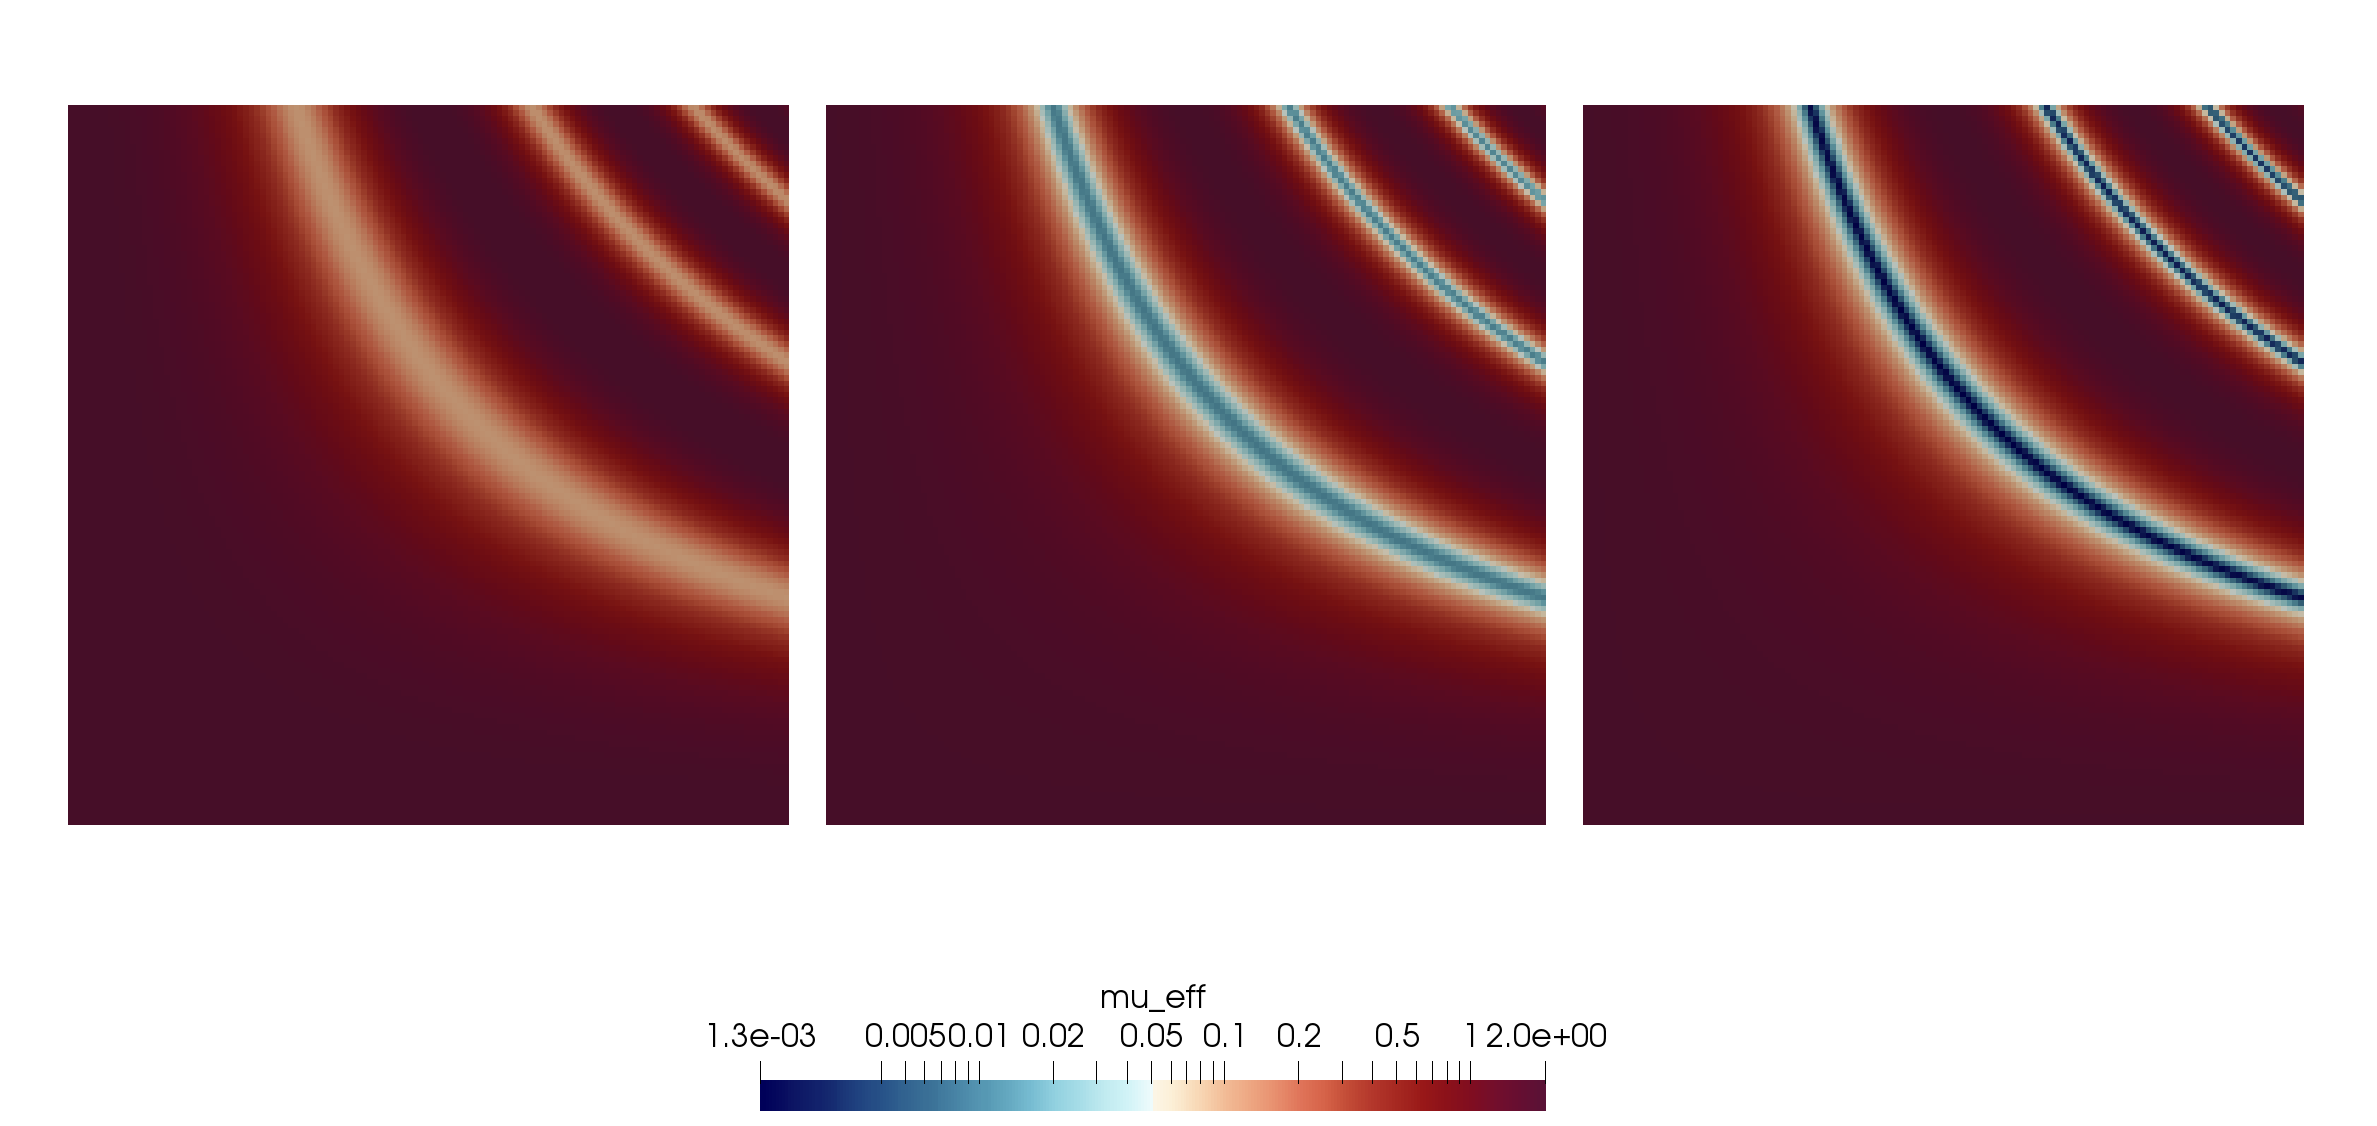
\includegraphics[width=14cm]{images/mms/mms7_mueffs}\\
Domain size 2x2 with $\epsilon=0.1, 0.01, 0.001$
\end{center}

Another interesting aspect of this benchmark is the fact that increasing the domain size
adds complexity to it as it increases the number of low viscosity zones and the spacing 
between them also decreases:

\begin{center}
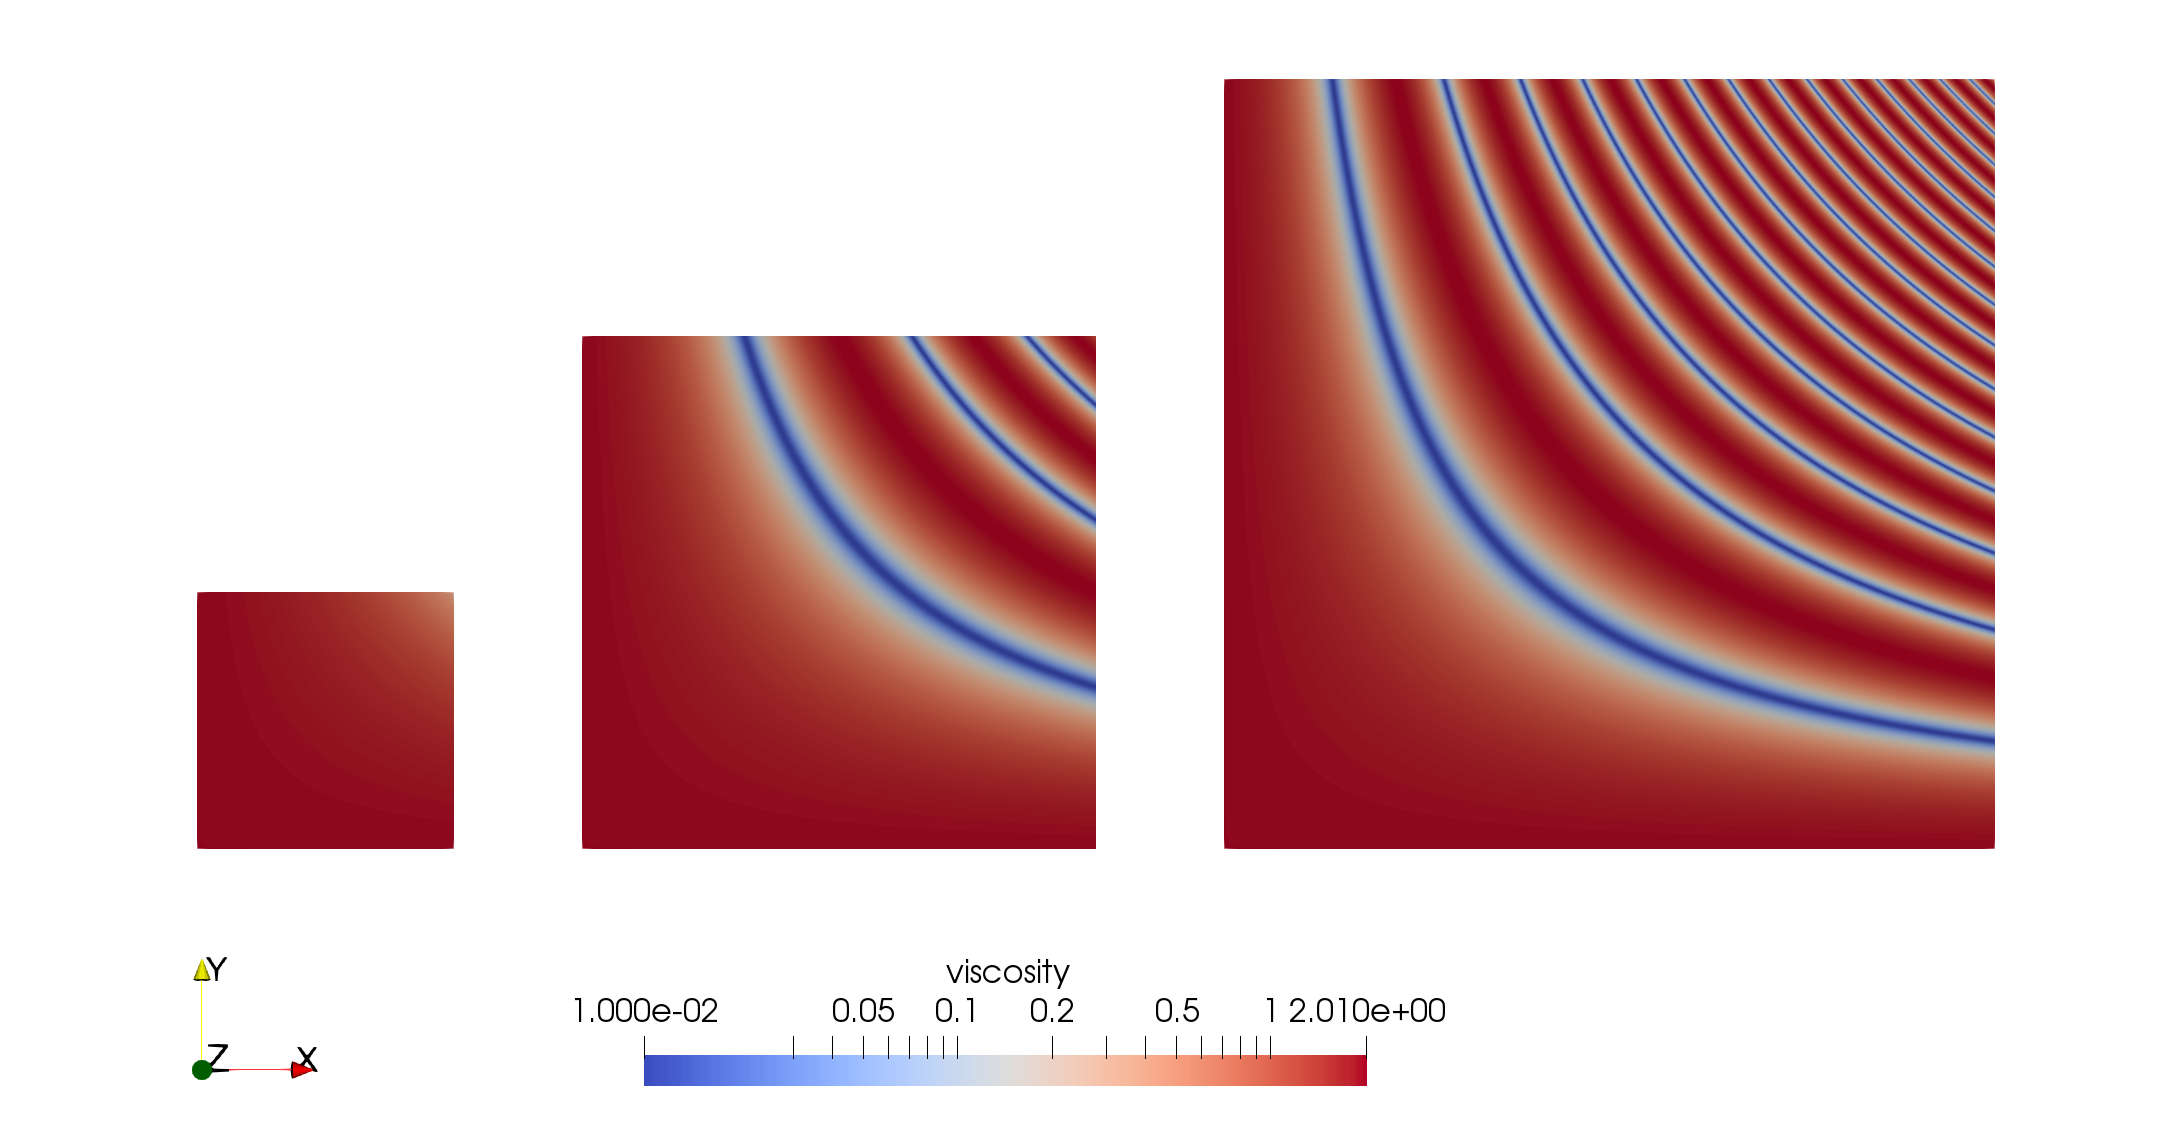
\includegraphics[width=7.28cm]{images/mms/mms7_visc}
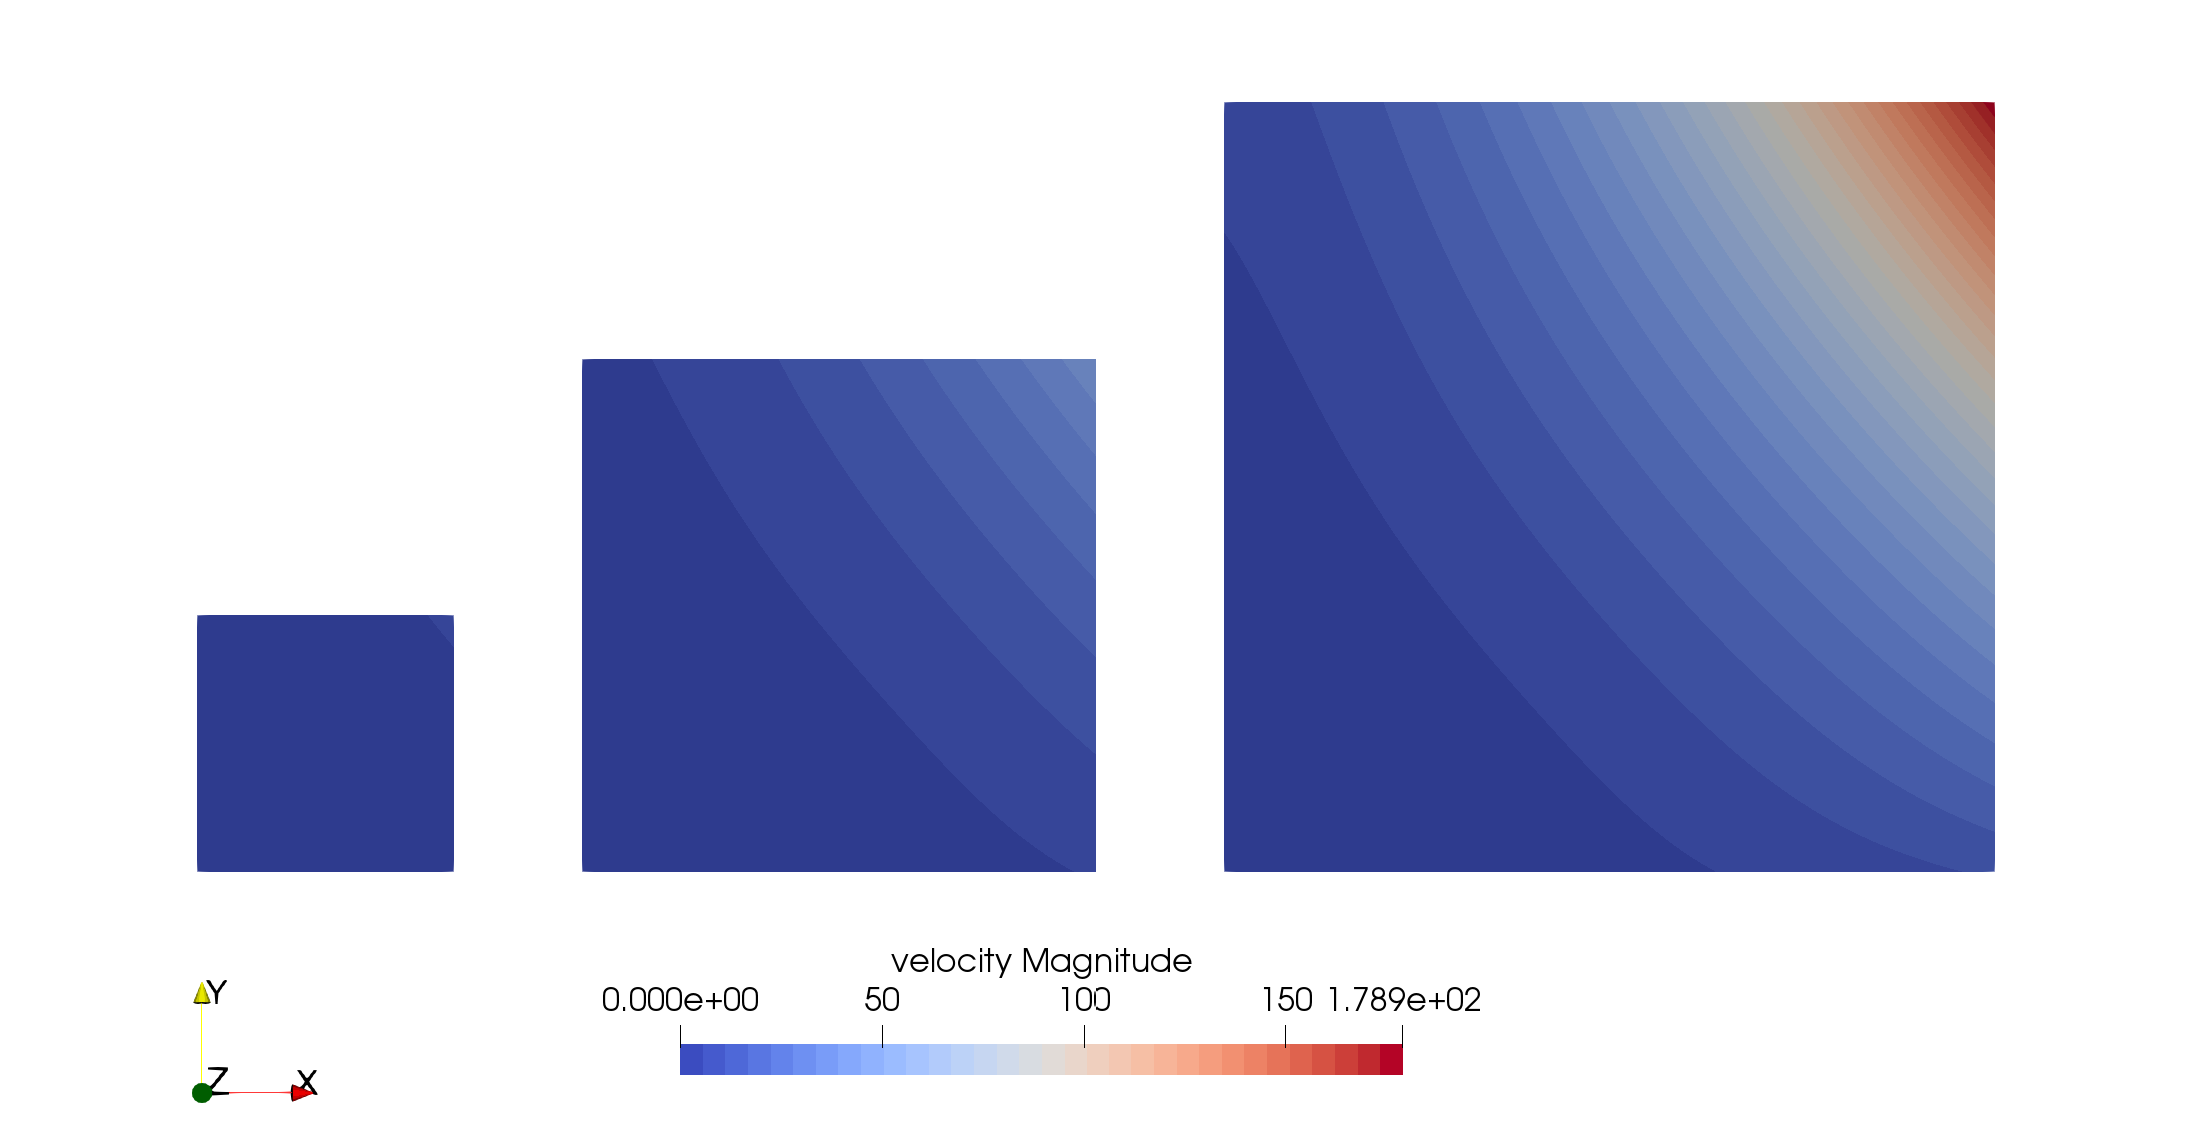
\includegraphics[width=7.28cm]{images/mms/mms7_vel}\\
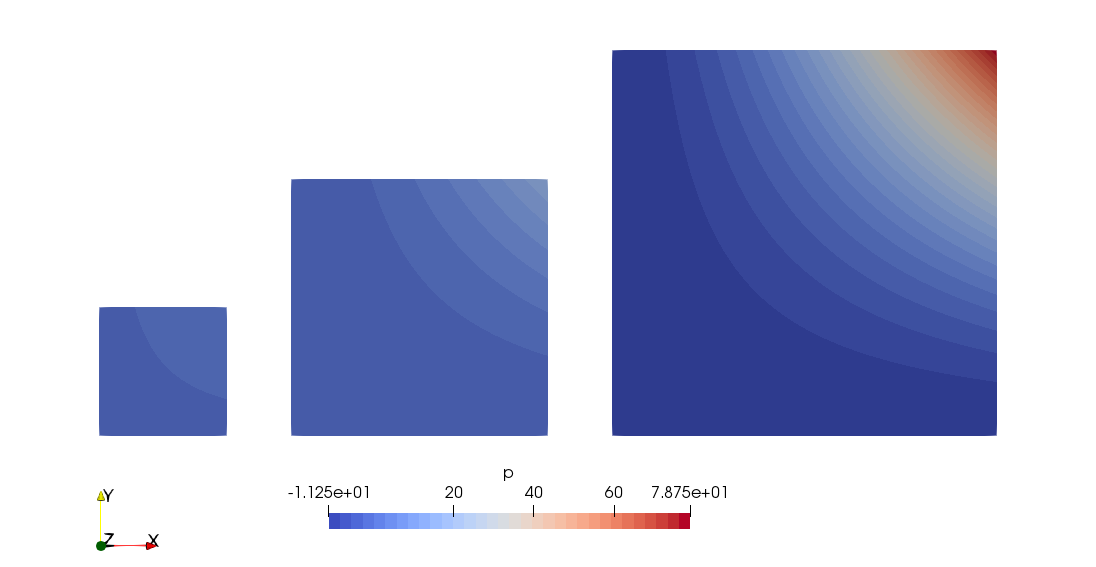
\includegraphics[width=7.28cm]{images/mms/mms7_press}
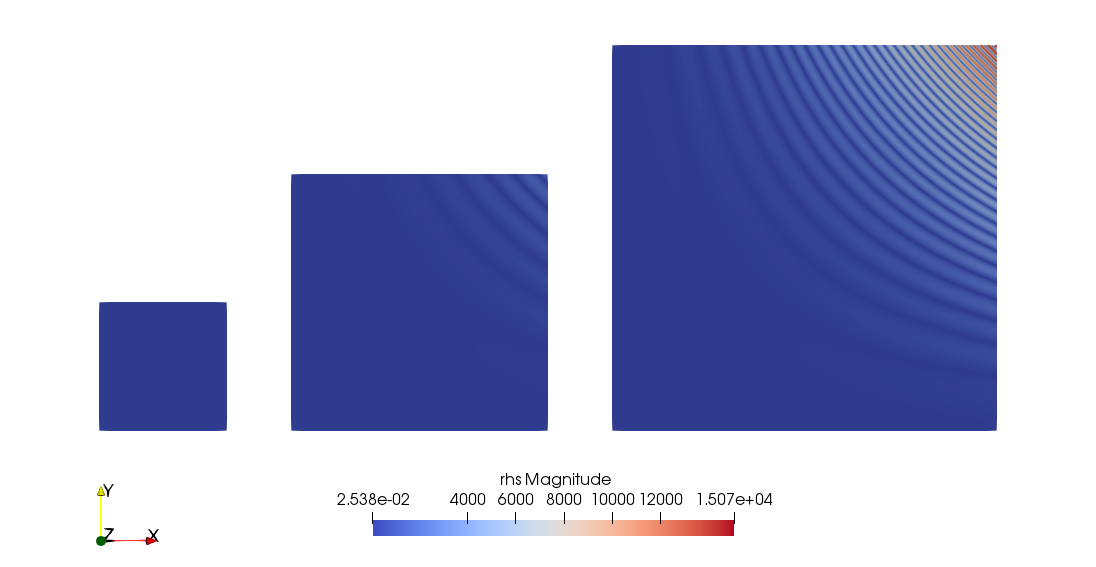
\includegraphics[width=7.28cm]{images/mms/mms7_rhs}\\
Three different domain sizes (1x1, 2x2, 3x3) with $\epsilon=0.001$.
\end{center}


Finally, because the analytical expression for both components of the velocity is a polynomial, we can also
compute the root mean square velocity exactly. For instance, for a 2x2 domain:
\begin{center}
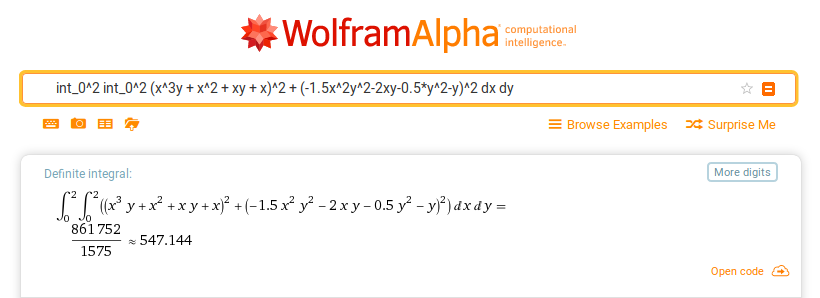
\includegraphics[width=8cm]{images/mms/mms7_vrmstheo}
\end{center}
and we end up with (for $L=2$)
\[
v_{rms} = \sqrt{\frac{1}{L^2}\frac{861752}{1575}} = \sqrt{\frac{215438}{1575}}
\simeq 11.6955560683
\]

\bscthesis \index{general}{BSc Thesis}

%-----------------------------------------------------------------------------
\subsubsection{Analytical benchmark VIII \label{mms8} - "Kovasznay"}

This flow was published by L.I.G. Kovasznay in 1948 \cite{kova48}. 
This paper presents an exact two-dimensional solution of the Navier-Stokes equations 
with a periodicity in the vertical direction, 
gives an analytical solution to the steady-state Navier-Stokes equations that is similar
which is a flow-field behind a periodic array of cylinders.

\begin{eqnarray}
u(x,y)&=&1-\exp(\lambda x) \cos (2\pi y)\\
v(x,y)&=&\frac{\lambda}{2\pi} \exp(\lambda x) \sin (2 \pi y)\\
p(x,y) &=& \frac{1}{2}(1-\exp (2\lambda x)) \\
\lambda&=&\frac{Re}{2}-\sqrt{\frac{Re^2}{4}+4\pi^2} 
\end{eqnarray}

Following step-55 of deal.II \footnote{\url{https://www.dealii.org/current/doxygen/deal.II/step_55.html}}
we have to 'cheat' here since we are not solving the non-linear Navier-Stokes equations, but the linear Stokes system without convective term. Therefore, to recreate the exact same solution
we move the convective term into the right-hand side.

The analytical solution is prescribed left and right, while free/no (??) slip is prescribed at top and bottom.

Velocity and pressure solution as implemented in step-55:
\begin{lstlisting}
const double pi2 = pi*pi;

u = -exp(x*(-sqrt(25.0 + 4*pi2) + 5.0))*cos(2*y*pi) + 1

v = (1.0L/2.0L)*(-sqrt(25.0 + 4*pi2) + 5.0)*
    exp(x*(-sqrt(25.0 + 4*pi2) + 5.0))*sin(2*y*pi)/pi

p = -1.0L/2.0L*exp(x*(-2*sqrt(25.0 + 4*pi2) + 10.0)) - 2.0*(-6538034.74494422 
  + 0.0134758939981709*exp(4*sqrt(25.0 + 4*pi2)))/(-80.0*exp(3*sqrt(25.0 + 4*pi2)) 
  + 16.0*sqrt(25.0 + 4*pi2)*exp(3*sqrt(25.0 + 4*pi2))) 
  - 1634508.68623606*exp(-3.0*sqrt(25.0 + 4*pi2))/(-10.0 + 2.0*sqrt(25.0 + 4*pi2)) 
  + (-0.00673794699908547*exp(sqrt(25.0 + 4*pi2)) 
  + 3269017.37247211*exp(-3*sqrt(25.0 + 4*pi2)))/(-8*sqrt(25.0 + 4*pi2) + 40.0) 
  + 0.00336897349954273*exp(1.0*sqrt(25.0 + 4*pi2))/(-10.0 + 2.0*sqrt(25.0 + 4*pi2))
\end{lstlisting}
while the rhs of the PDE is given by


\begin{lstlisting}
const double pi2 = pi * pi;

values[0] = -1.0L / 2.0L * (-2 * sqrt(25.0 + 4 * pi2) + 10.0) *
            exp(x*(-2*sqrt(25.0 + 4 * pi2) + 10.0)) -
            0.4 *pi2*exp(x * (-sqrt(25.0 + 4 * pi2) + 5.0)) * cos(2 * y * pi) +
            0.1 *pow(-sqrt(25.0 + 4 * pi2) + 5.0, 2) *
            exp(x*(-sqrt(25.0 + 4 * pi2) + 5.0)) * cos(2 * y * pi)

values[1] = 0.2 * pi*(-sqrt(25.0 + 4 * pi2) + 5.0) *
            exp(x*(-sqrt(25.0 + 4 * pi2) + 5.0)) * sin(2 * y * pi) -
            0.05 *pow(-sqrt(25.0 + 4 * pi2) + 5.0, 3) *
            exp(x*(-sqrt(25.0 + 4 * pi2) + 5.0)) * sin(2 * y * pi) / pi

values[2] = 0;
\end{lstlisting}

\begin{center}
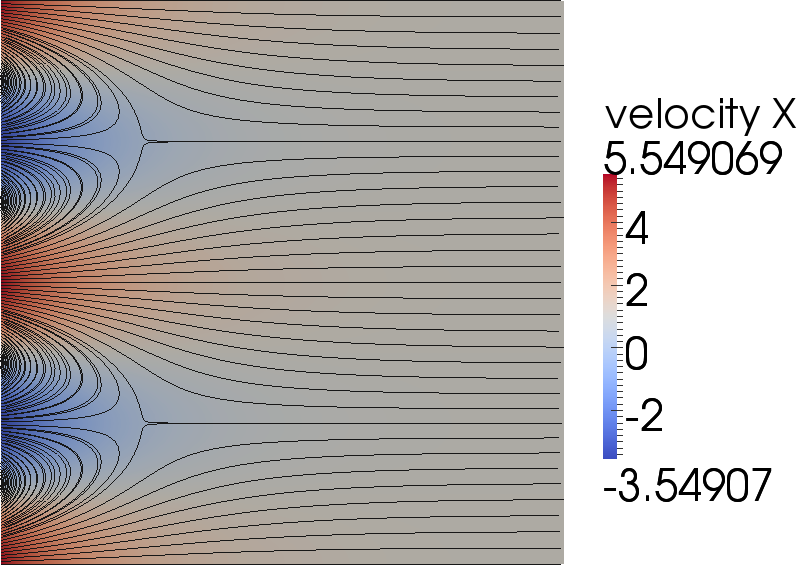
\includegraphics[width=5cm]{images/mms/kovasznay/step-55_solution}
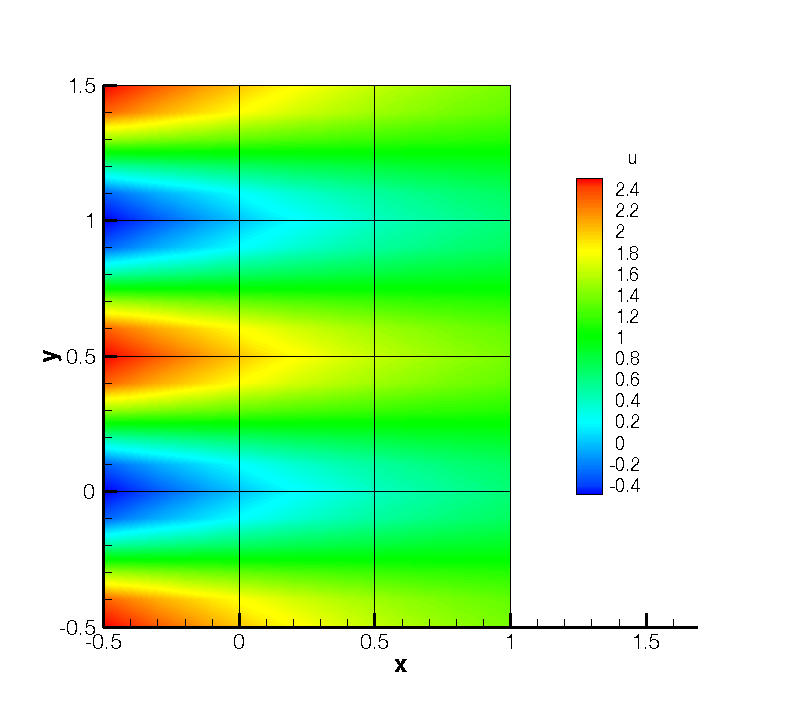
\includegraphics[width=5cm]{images/mms/kovasznay/KF2DCVP8}
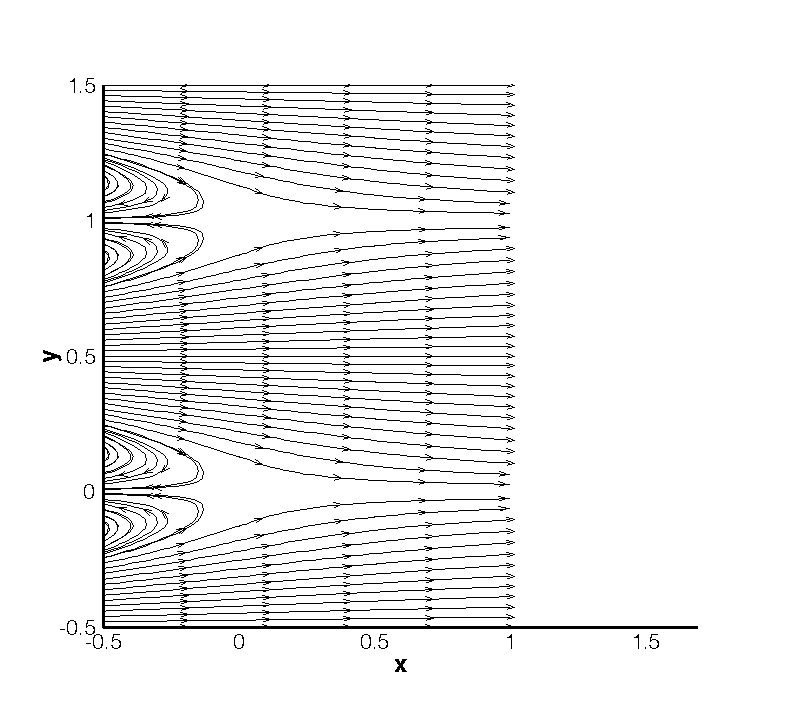
\includegraphics[width=5cm]{images/mms/kovasznay/KF2DCVP8SL}\\
{\captionfont 
Left: solution from Step-55. Right:
Solution obtained with 
NekTar++\footnote{\url{http://doc.nektar.info/userguide/4.3.4/user-guidese45.html}}}
\end{center}


This benchmark is carried out in many CFD papers: \cite{coks04b,bodi11,ngpe12}, see also Section 7.4.3
of Hesthaven \& Warburton \cite{hewa08}.

\todo[inline]{Find analytical expression for pressure. Compute expression for rhs. Make stone}

\bscthesis \index{general}{BSc Thesis}

%-----------------------------------------------------------------------------
\subsubsection{Analytical benchmark IX \label{mms9} - "VJ2"}

It is presented in \cite{jolm17} and meant to be a peculiar case where the velocity solution 
is exactly zero. The viscosity is 1, the domain is a unit square, no-slip boundary conditions 
are prescribed everywhere. The buoyancy force is given by $\vec{b}=(0,Ra(1-y+3y^2))$ where 
$Ra>0$ is a parameter. The flow is incompressible and the analytical pressure solution 
is given by $p=Ra(y^3-y^2/2+y-7/12)$.

%-----------------------------------------------------------------------------
\subsubsection{Analytical benchmark X \label{mms10} - "VJ3"}

This benchmark comes from John et al. \cite{jolm17}.
The domain is once again the unit square. The velocity field has the form of a large vortex.

\begin{eqnarray}
u(x,y) &=& 200x^2(1-x)^2y(1-y)(1-2y) \\
v(x,y) &=& -200x(1-x)(1-2x)y^2(1-y)^2 \\
p(x,y) &=& 10\left[(x-1/2)^3y^2+(1-x)^3(y-1/2)^3 \right]
\end{eqnarray}

\begin{center}
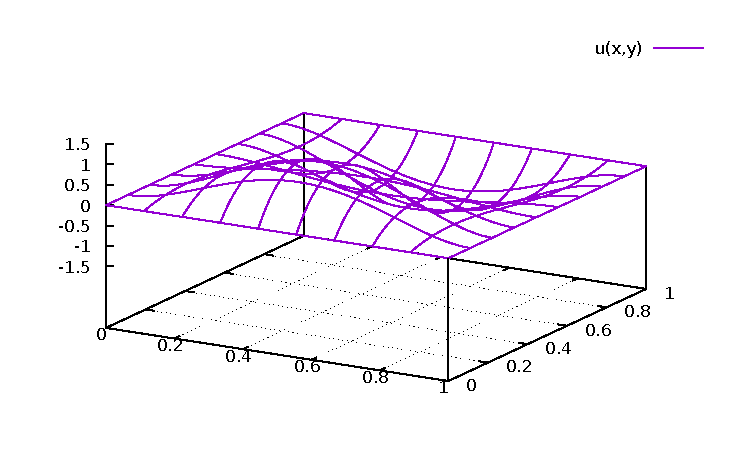
\includegraphics[width=4.5cm]{images/benchmark_VJ3/u.pdf}
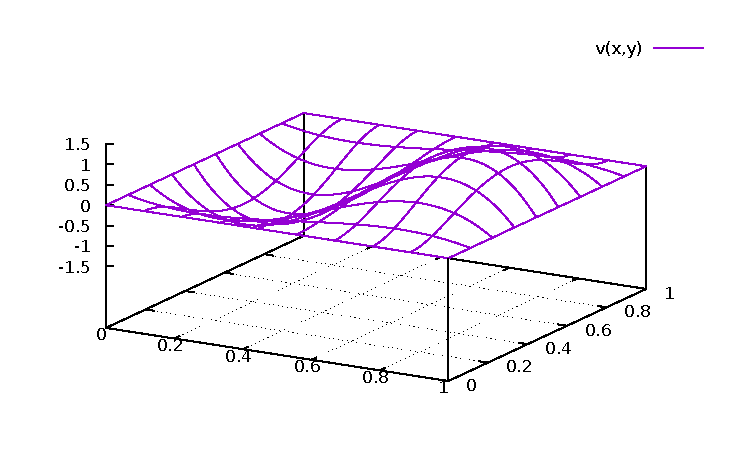
\includegraphics[width=4.5cm]{images/benchmark_VJ3/v.pdf}
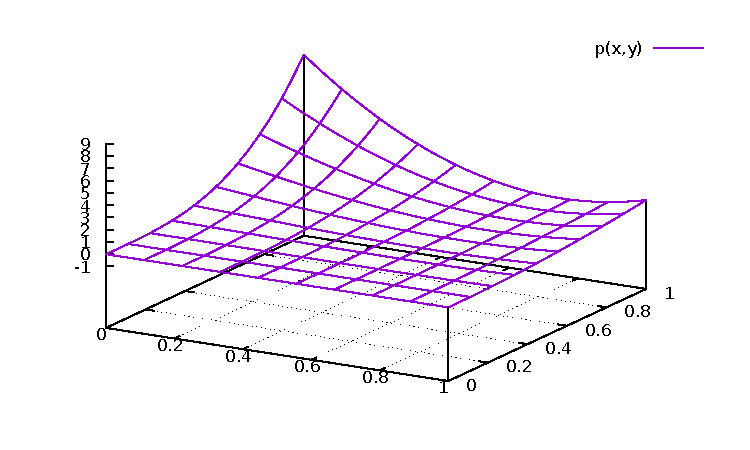
\includegraphics[width=4.5cm]{images/benchmark_VJ3/p.pdf}
\end{center}

\begin{eqnarray}
\dot{\varepsilon}_{xx}=\frac{\partial u}{\partial x} &=& -400(1-x)x(2x-1)(y-1)y(2y-1)  \\
\frac{\partial u}{\partial y} &=& 200(1-x)^2x^2 (6y^2-6y+1)  \\
\frac{\partial v}{\partial x} &=& -200(6x^2-6x+1)(1-y)^2y^2  \\
\dot{\varepsilon}_{yy}=\frac{\partial v}{\partial y} &=& 400(x-1)x(2x-1)(1-y)y(2y-1) 
\end{eqnarray}
so that 
\begin{eqnarray}
\dot{\varepsilon}_{xy}
&=&\frac{1}{2} \left[ 200(1-x)^2x^2 (6y^2-6y+1)   -200(6x^2-6x+1)(1-y)^2y^2  \right] \nn\\
&=&100(1-x)^2x^2 (6y^2-6y+1)   -100(6x^2-6x+1)(1-y)^2y^2 
\end{eqnarray}
Also
\begin{eqnarray}
\frac{\partial \dot{\varepsilon}_{xx}}{\partial x} &=& 400(6x^2-6x+1)y(2y^2-3y+1) \nn\\
\frac{\partial \dot{\varepsilon}_{xy}}{\partial x} 
&=& 200 (-2 x^2 (1 - x) (6 y^2 - 6 y + 1) + 2 x (1 - x)^2 (6 y^2 - 6 y + 1) - 6 (2 x - 1) (1 - y)^2 y^2)\nn\\
&=&  100 (-2 x^2 (1 - x) (6 y^2 - 6 y + 1) + 2 x (1 - x)^2 (6 y^2 - 6 y + 1) - 6 (2 x - 1) (1 - y)^2 y^2) \nn\\
\frac{\partial \dot{\varepsilon}_{xy}}{\partial y} &=& 400 (6 x^2 - 6 x + 1) (1 - y) y^2 + 200 (1 - x)^2 x^2 (12 y - 6) - 400 (6 x^2 - 6 x + 1) (1 - y)^2 y   \nn \\
\frac{\partial \dot{\varepsilon}_{yy}}{\partial y} &=& -400x(2x^2-3x+1)(6y^2-6y+1) 
\end{eqnarray}


\begin{eqnarray}
\frac{\partial p}{\partial x} &=& 30(x-1/2)^2y^2-30(1-x)^2(y-1/2)^3 \\
\frac{\partial p}{\partial y} &=& 20(x-1/2)^3y + 30(1-x)^3(y-1/2)^2  
\end{eqnarray}

From $\vec\nabla\cdot{\bm \sigma}+\vec{b}=\vec{0}$ we can obtain the rhs as follows:
\begin{eqnarray}
\vec{b} 
&=& - \vec\nabla\cdot{\bm \sigma} \nn\\ 
&=& \vec\nabla p -  \vec\nabla\cdot{\bm s} \nn\\ 
&=& \vec\nabla p -  \vec\nabla\cdot(2 \eta \dot{\bm \varepsilon})  
\end{eqnarray}
Assuming $\eta=1$ we arrive at:
\begin{eqnarray}
b_x &=&  \frac{\partial p}{\partial x} 
-2\frac{\partial \dot{\varepsilon}_{xx}}{\partial x}  
-2\frac{\partial \dot{\varepsilon}_{xy}}{\partial y}  \\
b_y &=&  \frac{\partial p}{\partial y}  
-2\frac{\partial \dot{\varepsilon}_{xy}}{\partial x} 
-2\frac{\partial \dot{\varepsilon}_{yy}}{\partial y}  
\end{eqnarray}

All the necessary functions to do this benchmark are in {\tt mms/vj3.py}:
\lstinputlisting[language=python]{mms/vj3.py}

\begin{center}
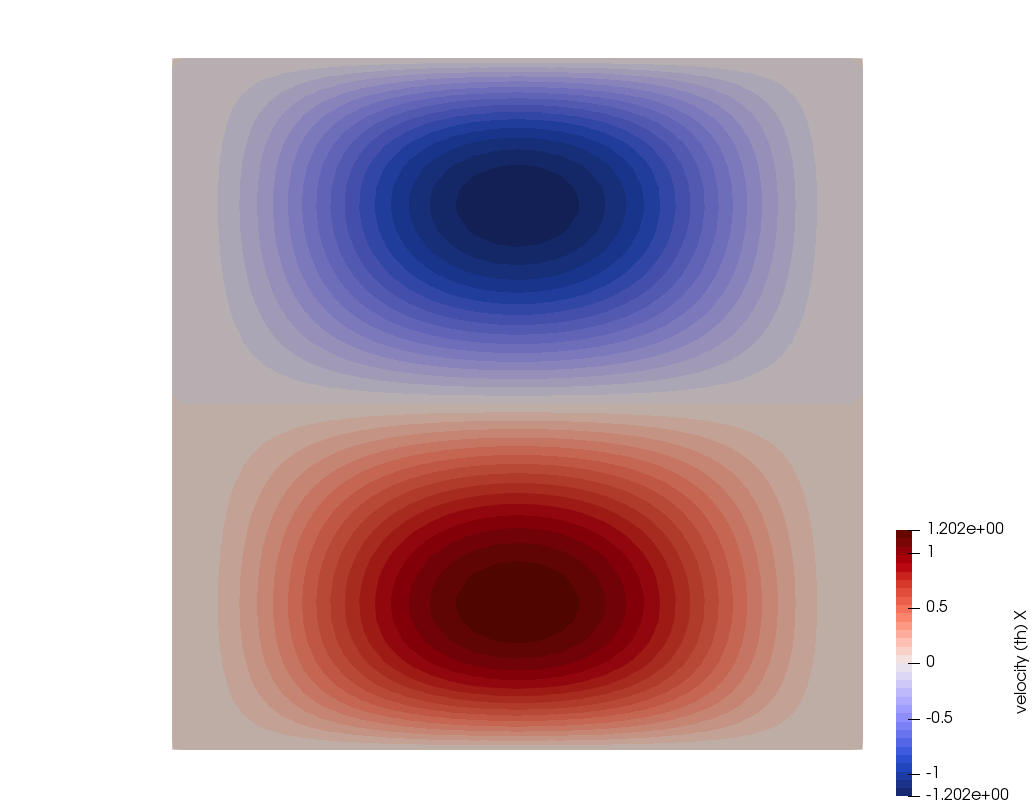
\includegraphics[width=4.5cm]{images/mms/vj3/u}
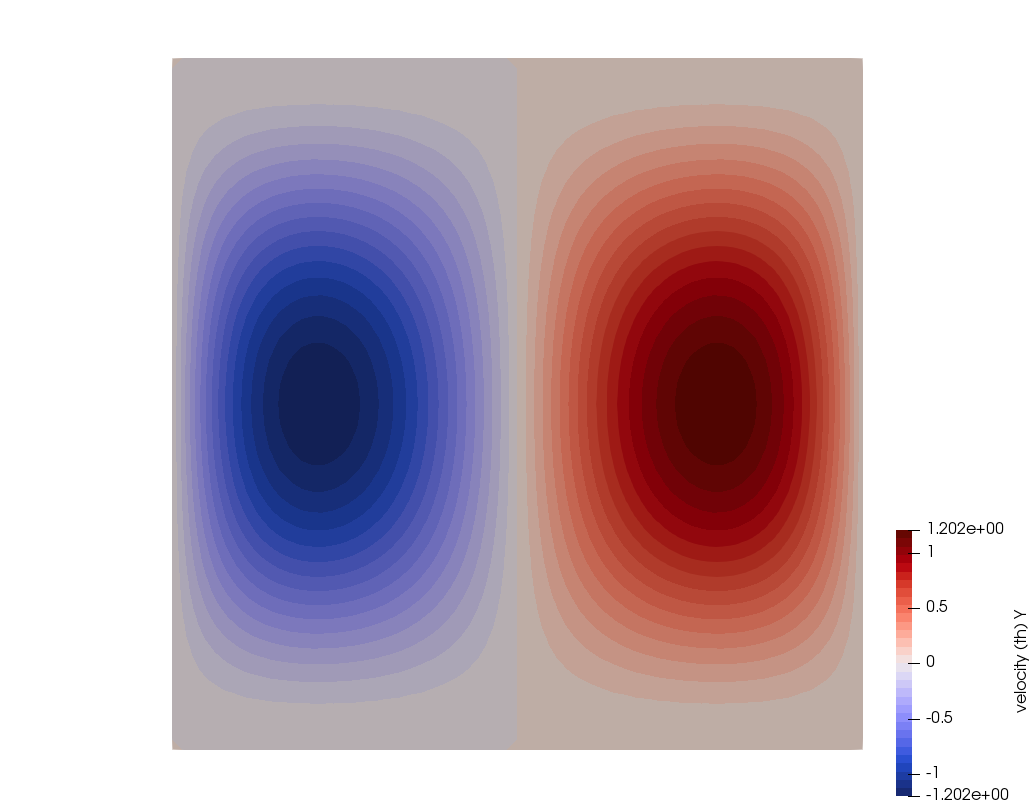
\includegraphics[width=4.5cm]{images/mms/vj3/v}
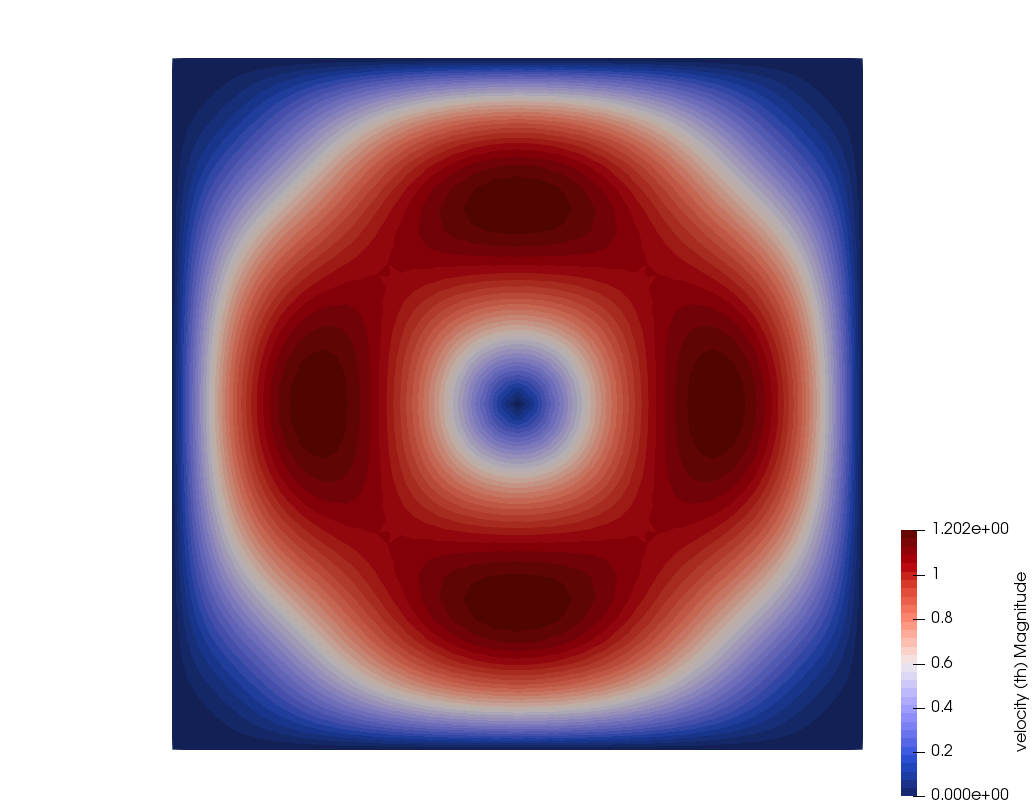
\includegraphics[width=4.5cm]{images/mms/vj3/vel}\\
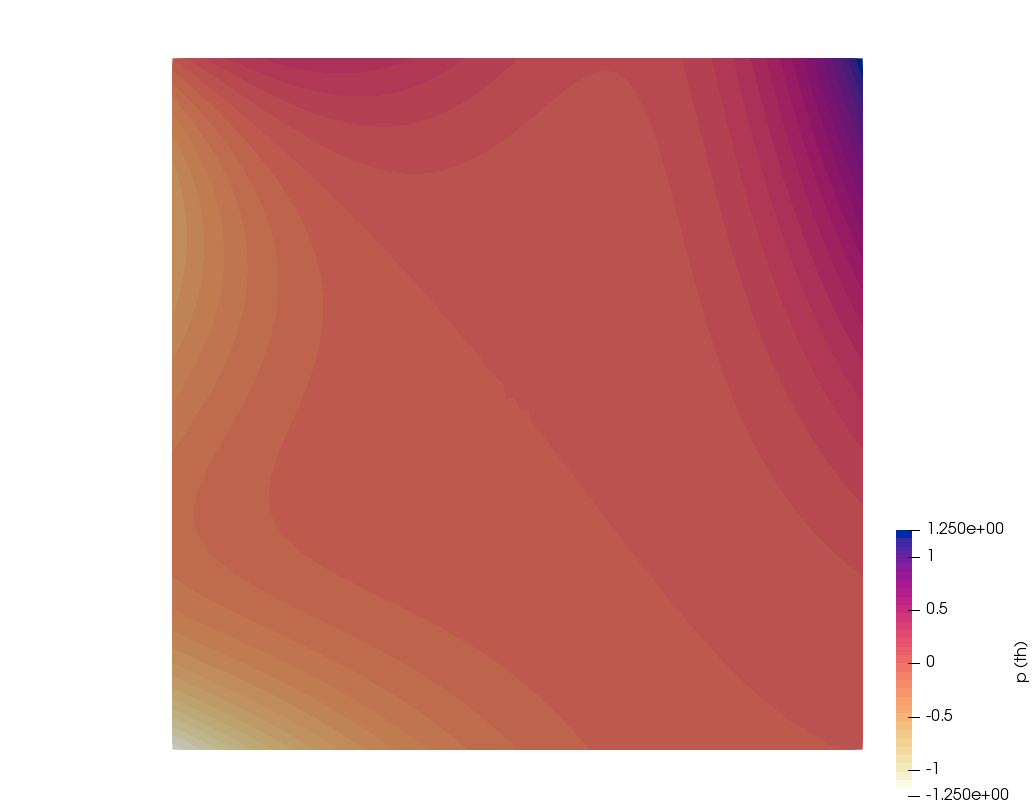
\includegraphics[width=4.5cm]{images/mms/vj3/p}
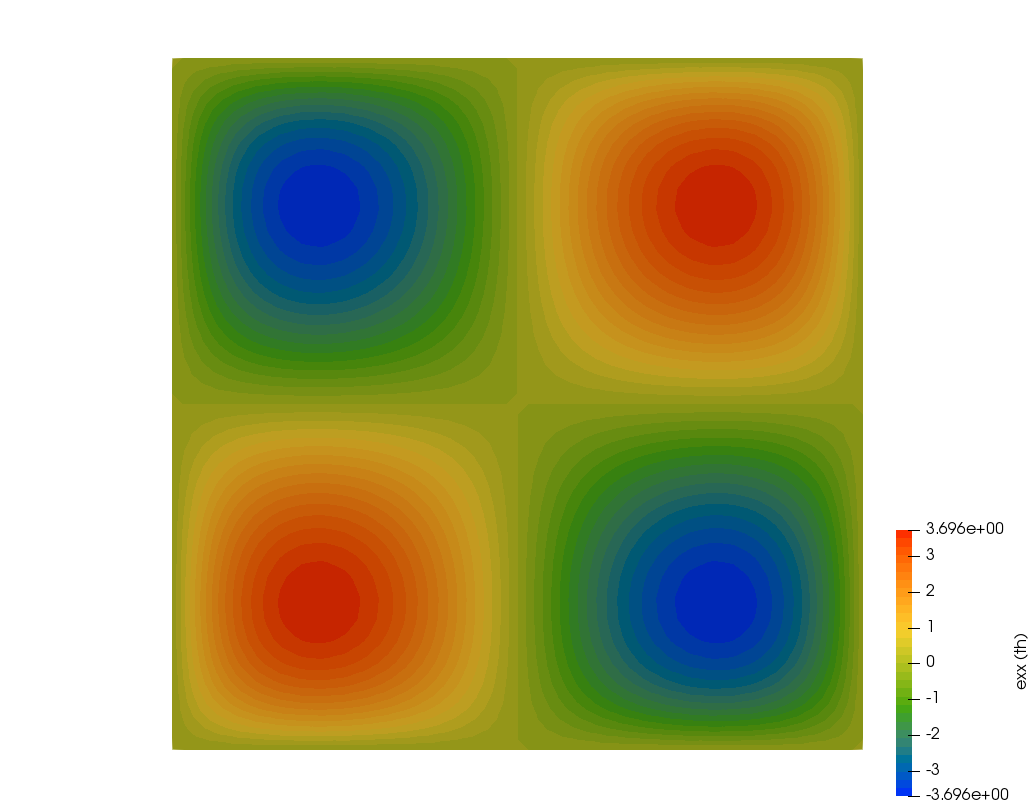
\includegraphics[width=4.5cm]{images/mms/vj3/exx}
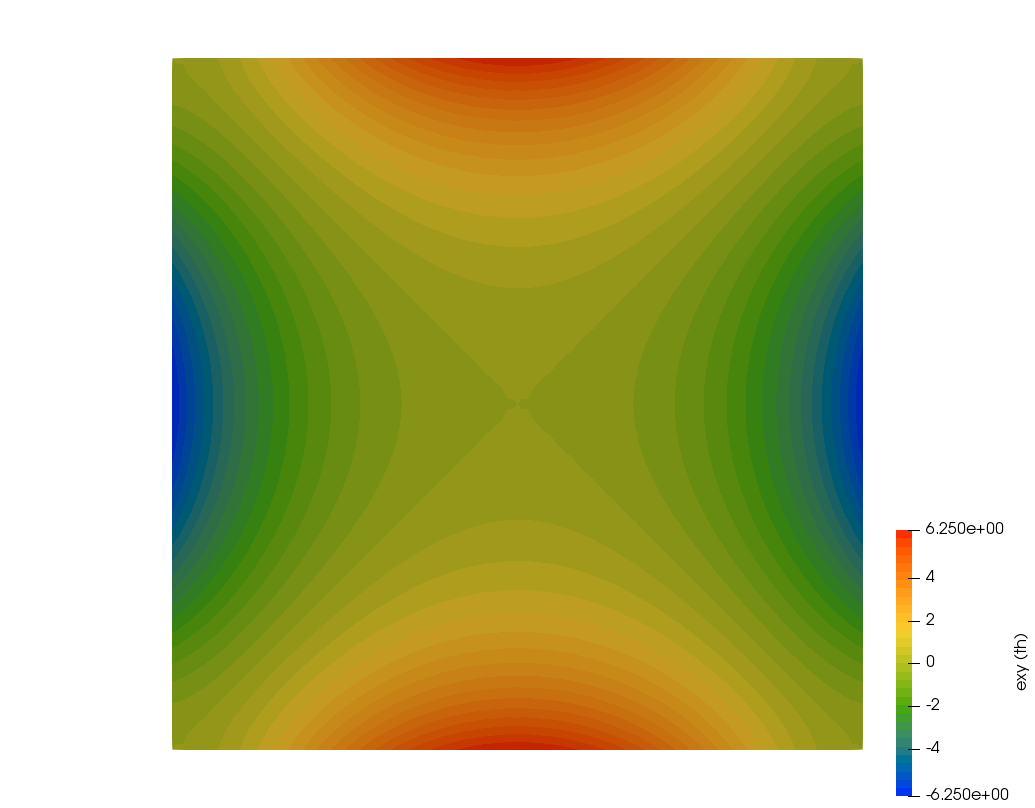
\includegraphics[width=4.5cm]{images/mms/vj3/exy}
\end{center}

%-----------------------------------------------------------------------------
%\subsubsection{Analytical benchmark XI \label{mms11} - "PPC1"}



%-----------------------------------------------------------------------------
%\subsubsection{Analytical benchmark XII \label{mms12} - "PPC2"}


%-----------------------------------------------------------------------------
\subsubsection{Analytical benchmark XI \label{ss:mms11} - "LAMI"}

Taken from Lamichhane (2017) \cite{lami17}.

\begin{eqnarray}
u(x,y)&=&-2x^2y(2y-1)(x-1)^2(y-1) = a(x)b(y)\\
v(x,y)&=& 2xy^2(2x-1)(x-1)(y-1)^2 = c(x)d(y)\\
p(x,y)&=& x(1-x)(1-2y)
\end{eqnarray}
with
\begin{eqnarray}
a(x)&=&-2x^2(x-1)^2  \\
b(y)&=& y(2y-1)(y-1) \\ 
c(x)&=& x(2x-1)(x-1) \\
d(y)&=& 2y^2(y-1)^2
\end{eqnarray}
and 
\begin{eqnarray}
a'(x) &=&  -4x(2x^2-3x+1)\\
a''(x)&=&  -4(6x^2-6x+1) \\
b'(y) &=&  6y^2-6y+1 \\
b''(y)&=&  12y-6 \\
c'(x) &=& 6x^2-6x+1 \\
c''(x)&=& 12x-6  \\
d'(y) &=& 4y(2y^2-3y+1)  \\
d''(y)&=&  4(6y^2-6y+1)  
\end{eqnarray}



It then follows:
\begin{eqnarray}
{L}_{xx} &=& \frac{\partial u}{\partial x} =a'(x) b(y)\\ 
{L}_{xy} &=& \frac{\partial v}{\partial x} =c'(x) d(y)\\
{L}_{yx} &=& \frac{\partial u}{\partial y} =a(x) b'(y)\\
{L}_{yy} &=& \frac{\partial v}{\partial y} =c(x) d'(y)
\end{eqnarray}

It then follows:
\begin{eqnarray}
\dot{\varepsilon}_{xx} &=& L_{xx} = a'(x) b(y) \\
\dot{\varepsilon}_{yy} &=& L_{yy} = c(x) d'(y) \\
\dot{\varepsilon}_{xy} 
&=& \frac{1}{2} (L_{xy}+L_{yx}) \\
&=& \frac{1}{2} ( a(x) b'(y) +  c'(x) d(y)   ) 
\end{eqnarray}

We easily verify that $\dot{\varepsilon}_{xx}+\dot{\varepsilon}_{yy}=0$.

\begin{eqnarray}
\frac{\partial p}{\partial x} &=& (1-2x)(1-2y)\\
\frac{\partial p}{\partial y} &=& -2 x(1-x) 
\end{eqnarray}

We will also need:
\begin{eqnarray}
\frac{\partial \dot{\varepsilon}_{xx}}{\partial x}  &=& a''(x) b(y) \\
\frac{\partial \dot{\varepsilon}_{xy}}{\partial y}  &=& \frac{1}{2} ( a(x) b''(y) +  c'(x) d'(y)   )\\
\frac{\partial \dot{\varepsilon}_{xy}}{\partial x}  &=& \frac{1}{2} ( a'(x) b'(y) +  c''(x) d(y)   ) \\
\frac{\partial \dot{\varepsilon}_{yy}}{\partial x}  &=& c(x) d''(y)
\end{eqnarray}

Assuming $\eta=1$ we arrive at:
\begin{eqnarray}
b_x 
&=&  \frac{\partial p}{\partial x} 
-2\frac{\partial \dot{\varepsilon}_{xx}}{\partial x}  
-2\frac{\partial \dot{\varepsilon}_{xy}}{\partial y}  \\
&=&  (1-2x)(1-2y) - 2a''(x) b(y) - ( a(x) b''(y) +  c'(x) d'(y)   ) \\
b_y 
&=&  \frac{\partial p}{\partial y}  
-2\frac{\partial \dot{\varepsilon}_{xy}}{\partial x} 
-2\frac{\partial \dot{\varepsilon}_{yy}}{\partial y} \\
&=& -2 x(1-x) - ( a'(x) b'(y) +  c''(x) d(y)   ) -2  c(x) d''(y)
\end{eqnarray}

We have (thank you WolframAlpha\footnote{\url{https://www.wolframalpha.com/}}):
\[
\int_{0}^{1}\int_{0}^{1} u^2 dxdy= 
\int_{0}^{1}\int_{0}^{1} 
( -2x^2y(2y-1)(x-1)^2(y-1) )^2 
dxdy = \frac{1}{33075}
\]
\[
\int_{0}^{1}\int_{0}^{1} v^2 dxdy= 
\int_{0}^{1}\int_{0}^{1} 
( 2xy^2(2x-1)(x-1)(y-1)^2 )^2
dxdy = \frac{1}{33075}
\]
so that
\[
v_{rms} = \sqrt{\frac{1}{L_xL_y} \frac{2}{33075}  }
\simeq 0.00777615791
\]

Finally we can verify that the pressure has zero average:
\[
\int_0^1 \int_0^1 p(x,y) dx dy = 
\int_0^1 \int_0^1  x(1-x)(1-2y) dxdy= 
\int_0^1  x(1-x) dx \int_0^1  (1-2y) dy=0 
\]


%-----------------------------------------------------------------------------
\subsubsection{Annulus with kinematical b.c. - pure rotation} \label{ss:ankbc}

The domain is a hollow cylinder or inner radius $R_{i}$ and outside radius $R_{o}=1$.
Boundary conditions are prescribed both on the inside and the outside with 
${\vec \upnu}=(u,v)=(-y,x)$, or in 
polar coordinates ${\vec \upnu}=r {\vec e}_\theta$.

The gravity is radial and is set to
\[
g_x=-x/r  \quad\quad g_z=-y/r
\]
where $r=\sqrt{x^2+z^2}$, which in polar coordinates is ${\vec g}=-{\vec e}_r$.
The viscosity is also set to 1, and the density is given by
\[
\rho(r)=r^n
\]
where $n$ is a positive or nul integer. The pressure is set to zero at the outer boundary.

The gradient operator in polar coordinates writes:
\[
{\vec \nabla} = \frac{\partial }{\partial r} {\vec e}_r 
+ \frac{1}{r} \frac{\partial }{\partial \theta} {\vec e}_\theta 
\]
and the Laplacian operator:
\[
\Delta = \frac{\partial^2}{\partial r^2} + \frac{1}{r} \frac{\partial }{\partial r} + \frac{1}{r^2} \frac{\partial^2 }{\partial \theta^2}
\]
Note that in our case we need to take the Laplacian of a vector, and unfortunately the Laplacian of a vector is not the Laplacian 
of the vector's coordinates in polar coordinates (unlike cartesian coordinates). 
The Laplacian of a vector is given by\footnote{\url{https://en.wikipedia.org/wiki/Vector\_Laplacian}} 
\[
\nabla^2 \vec{A} = \nabla(\nabla\cdot\vec{A}) - \nabla\times(\nabla \times\vec{A})
=
\left(
\begin{array}{l}
\frac{\partial^2 A_r}{\partial r^2} + \frac{1}{r} \frac{\partial A_r}{\partial r} - \frac{1}{r^2} A_r  + \frac{1}{r^2} \frac{\partial^2 A_r}{\partial \theta^2}  - \frac{2}{r^2} \frac{\partial A_\theta}{\partial \theta} \\ \\
\frac{\partial^2 A_\theta}{\partial r^2} + \frac{1}{r} \frac{\partial A_\theta}{\partial r} - \frac{1}{r^2} A_\theta  + \frac{1}{r^2} \frac{\partial^2 A_\theta}{\partial \theta^2}  + \frac{2}{r^2} \frac{\partial A_r}{\partial \theta} 
\end{array}
\right)
=
\left(
\begin{array}{l}
\Delta A_r \\ \\ \Delta A_\theta
\end{array}
\right)
\]
The Stokes equation writes:
\[
-\vec\nabla p + \eta \Delta {\vec \upnu} + \rho {\vec g} = {\vec 0}
\]
The velocity solution is expected to be ${\vec \upnu}= r {\vec e}_\theta $.
The Stokes equation in polar coordinates then writes:
\[
-\frac{\partial p}{\partial r} + \Delta v_r + \rho(r) (- 1)  = 0 
\]
\[
-\frac{1}{r}\frac{\partial p}{\partial \theta} + \Delta v_\theta = 0
\]
Since $\Delta v_\theta = 0$, then $\frac{\partial p}{\partial \theta}=0$ and then the pressure is independent of $\theta$, 
which is what we expect since the density distribution is radial. 
We then focus on the first equation, and since $v_r=0$, we then obtain:
\[
\frac{\partial p}{\partial r}  = - \rho(r)
\]

\begin{itemize}
\item If $\rho(r)=1$, then 
\[
\frac{\partial p}{\partial r}  = - 1
\]
yields $p(r)=-r+C$ where C is a constant determined by means of b.c. ($p(r=1)=0$) so finally
\[
\boxed{
p(r)=1-r
}
\]

\item If $\rho(r)=r$, then 
\[
\frac{\partial p}{\partial r}  = - r
\]
so that $p(r)=-\frac{1}{2}r^2 + C$ and likewise
\[
\boxed{
p(r)=\frac{1}{2} (1- r^2)
}
\]
\end{itemize}
  
In general, by taking $\rho(r)=r^n$ with $n=0,1,...$ one arrives to a pressure field given by 
\[
\boxed{
p(r)=\frac{1}{n+1} (1- r^{n+1})
}
\]

\begin{center}
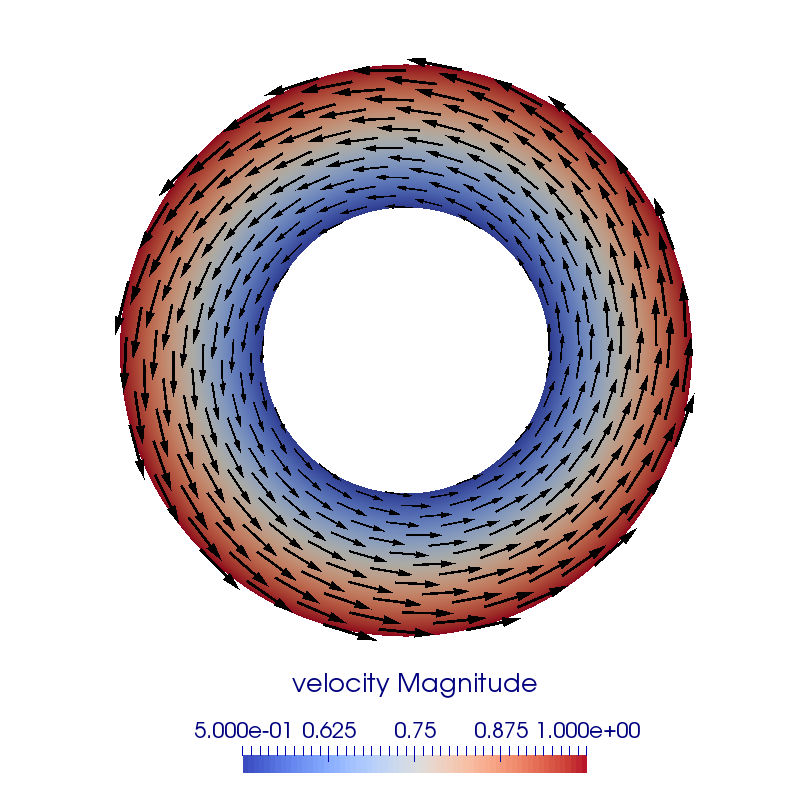
\includegraphics[width=6cm]{images/benchmark_annulus_mms/vel}
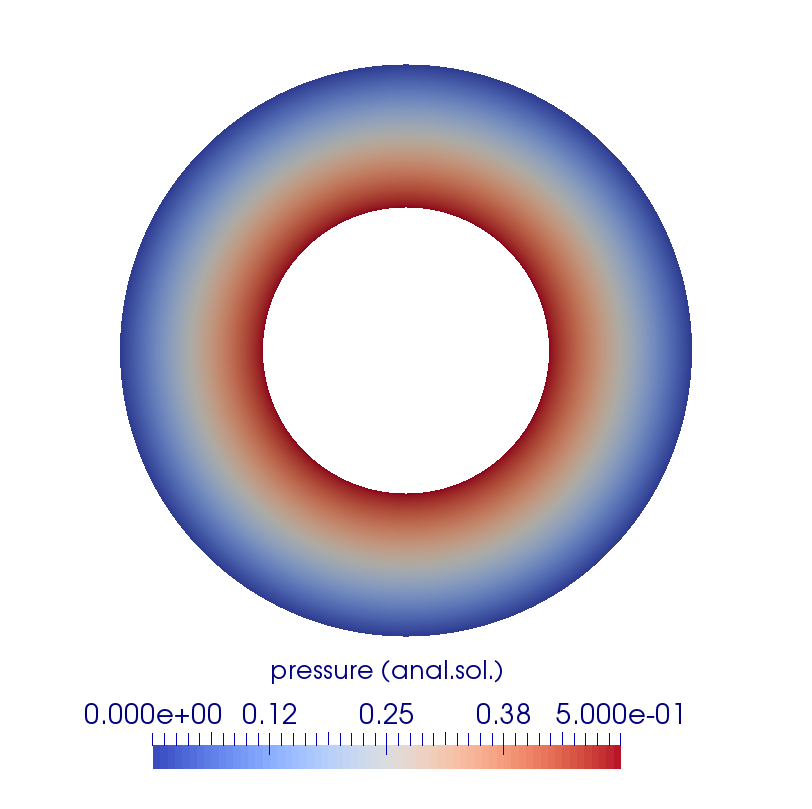
\includegraphics[width=6cm]{images/benchmark_annulus_mms/press}
\end{center}

This benchmark is of course very simple and the fact that the solution is independent of $\theta$
renders it not so useful. It has succesfully been implemented in \elefant.

%-----------------------------------------------------------------------------
\subsubsection{Viscous beam under extension}

The domain is a Cartesian box of size $L_x \times L_y$. 
Velocity $-u_0$ is applied on the left boundary and 
velocity $+u_0$ is applied on the right boundary. 
Bottom and top boundaries are left free. 
If no vertical velocity is prescribed anywhere there is an obvious nullspace 
in the solution which is problematic (numerically of course, but also 
because the solution is then not unique). One might want to set $v=0$ at $y=L_y/2$
on each side for example. 
The solution to this problem (incompressible Stokes equations) is given by
\begin{eqnarray}
u(x,y)&=&2u_0(x/L_x-1/2)\\
v(x,y)&=&-2 u_0 L_y/L_x (y/L_y-1/2)
\end{eqnarray}
in the absence of gravity. The strain rate tensor is then:
\[
\dot{\bm \varepsilon} =
\left(
\begin{array}{cc}
\dot{\varepsilon}_{xx} & \dot{\varepsilon}_{xy} \\
\dot{\varepsilon}_{xx} & \dot{\varepsilon}_{yy} 
\end{array}
\right)
=
\left(
\begin{array}{cc}
2 u_0 /Lx & 0 \\
0 & -2 u_0 /L_x 
\end{array}
\right)
\]
and we see that the flow is indeed incompressible as the trace 
of the strain rate tensor is zero. 

The momentum equation is 
\[
-\vec\nabla p + \vec\nabla \cdot (2 \eta \dot{\bm\varepsilon}) = \rho \vec g
\]
where the viscosity $\eta$ is constant in space. 
If gravity is set to zero, we obtain:
\begin{eqnarray}
-\frac{\partial p}{\partial x} &=& 0 \\
-\frac{\partial p}{\partial y} &=& 0 
\end{eqnarray}
since the strain rate is constant in space and the divergence operator applied to it returns 
the zero tensor. We there fore can conclude that pressure should be constant. 

Since the top and bottom boundaries are free, we have ${\bm \sigma}\cdot \vec{n} = \vec{0}$ on these.
The stress tensor is given by ${\bm \sigma} = - {\bm 1} + 2 \eta \dot{\bm \varepsilon}$ and the normal on the 
top is $\vec{n}=(0,+1)$ so that on the top boundary we have
\[
- p + 2 \eta \dot{\epsilon}_{yy} = 0
\]
or, 
\[
p= 2 \eta \dot{\epsilon}_{yy} 
\]
Note that using the bottom boundary with $\vec{n}=(0,-1)$ yields the same result.


\newpage
%-----------------------------------------------------------------------------
\subsubsection{Channel flow with Herschel-Bulkley rheology \label{ss:HBflow}}

We start from the following formulation for the Herschel-Bulkley rheology:
\begin{mdframed}[backgroundcolor=blue!5]
\[
\eta_{HB}
=
\left\{
\begin{array}{lc}
\eta_0 & \dot{\varepsilon}_e\leq \dot{\varepsilon}_0 \\
K  \dot{\varepsilon}_e^{n-1} + \frac{\tau_0}{\dot{\varepsilon}_e}  
& \dot{\varepsilon}_e\geq \dot{\varepsilon}_0 
\end{array}
\right.
\]
\end{mdframed}
and the limiting viscosity $\eta_0$ is such that 
\[
\eta_0 = K  \dot{\varepsilon}_0^{n-1} + \frac{\tau_0}{\dot{\varepsilon}_0}  
\]

We consider a two-dimensional channel in the $x,y$ plane. The walls 
are at $y=0$ and $y=H$ with no-slip boundary conditions. 
In the absence of gravity, the Stokes equation simplify to 
\begin{equation}
-\frac{\partial p}{\partial x}  +\frac{\partial }{\partial y} (2\eta_{HB} \dot{\varepsilon}_{xy}) =0
\qquad
\text{and}
\qquad
\dot{\varepsilon}_{xy} = \frac{1}{2} \frac{\partial u}{\partial y} 
\label{eq:hb1}
\end{equation}
where we assume the velocity $\vec\upnu=(u(y),0)$.
It then follows that 
\[
\dot{\varepsilon}_{e} 
= \sqrt{{\cal I}_2(\dot{\bm \varepsilon})} 
=\sqrt{ \frac{1}{2} \dot{\bm \varepsilon} : \dot{\bm \varepsilon} }
=\sqrt{ 
\frac{1}{2}[(\dot{\varepsilon}_{xx})^2 + (\dot{\varepsilon}_{yy})^2 + (\dot{\varepsilon}_{zz})^2]  
+ (\dot{\varepsilon}_{xy})^2  
+ (\dot{\varepsilon}_{xz})^2  
+ (\dot{\varepsilon}_{yz})^2 
}
=\sqrt{\dot{\varepsilon}_{xy}^2 }
= \left|\frac{1}{2} \frac{\partial u}{\partial y}  \right|
\]
In the case of a Newtonian fluid, the analytical solution is 
known and the velocity profile is a parabola with zero velocity on the
walls and maximum velocity in the middle. 
Although the rheology of the fluid is non-linear we assume that a 
similar velocity profile is expected (although not described by a parabola).
We then expect three zones (and we assume that the fluid flows from left to right):
\begin{itemize}

%..............................
\item In the middle, where it is expected that $\frac{\partial u}{\partial y}=0$ (at least in one point)
because of symmetry. We also therefore expect $\dot{\varepsilon}_e\leq \dot{\varepsilon}_0$ in this region
so that $\eta_{HB}=\eta_0$. How thick this region is will be determined later. 

Eq.~\eqref{eq:hb1} must then be solved 
\begin{eqnarray}
\frac{\partial p}{\partial x}  
&=&\frac{\partial }{\partial y} \left(2\eta_{HB}  \frac{1}{2}\frac{\partial u}{\partial y} \right) 
= \eta_0 \frac{\partial^2 u}{\partial y^2}  
\end{eqnarray}

Let us call $\Pi=\frac{\partial p}{\partial x} <0$, then we must solve:
\[
\frac{\partial^2 u}{\partial y^2} = \frac{\Pi}{\eta_0} 
\]
The solution is then of the form
\[
\boxed{
u(y)|_{mid} = \frac{1}{2}\frac{\Pi}{\eta_0} y^2 + 2a y + b
}
\]
and 
\[
\boxed{
\dot{\varepsilon}_{xy}|_{mid}= \frac{1}{2} \frac{\Pi}{\eta_0}y  + a
}
\]
We will determine $a$ and $b$ later. 

%..............................
\item Near the bottom wall, with $\frac{\partial u}{\partial y}>0$ so that  
$\dot{\varepsilon}_{e} = +\frac{1}{2}\left( \frac{\partial u}{\partial y}  \right)$  
and $\dot{\varepsilon}_e\geq \dot{\varepsilon}_0 $. 
We solve Eq.~\eqref{eq:hb1} again, this time with the non-linear formulation of the viscosity: 
\begin{eqnarray}
\frac{\partial p}{\partial x}  
&=&\frac{\partial }{\partial y} \left( 2 \eta_{HB}  \frac{1}{2}\frac{\partial u}{\partial y} \right)  \nn\\
&=&2 \frac{\partial }{\partial y} \left[  
\left( K  \dot{\varepsilon}_e^{n-1} + \frac{\tau_0}{\dot{\varepsilon}_e}  
\right) \frac{1}{2}\frac{\partial u}{\partial y} \right] \nn\\
&=&2\frac{\partial }{\partial y} \left[  
\left( K \left|\frac{1}{2}\frac{\partial u}{\partial y}\right|^{n-1} 
+ \tau_0 \left|\frac{1}{2}\frac{\partial u}{\partial y}\right|^{-1} 
\right) \frac{1}{2}\frac{\partial u}{\partial y} \right]  \nn\\
&=& 2 \frac{\partial }{\partial y} \left[  
K \left(\frac{1}{2}\frac{\partial u}{\partial y}\right)^{n} + \tau_0 \right] 
\end{eqnarray}
We then must solve:
\[
\frac{\partial }{\partial y} \left[  
K \left(\frac{1}{2}\frac{\partial u}{\partial y}\right)^{n} + \tau_0 \right] 
= \frac{\Pi}{2}
\]
\[
K \left(\frac{1}{2}\frac{\partial u}{\partial y}\right)^{n} + \tau_0  = \frac{\Pi}{2} y +c
\]
\[
\left(\frac{1}{2}\frac{\partial u}{\partial y}\right)^{n}   = \frac{1}{K} ( \frac{\Pi}{2} y +c -\tau_0 )
\]
or, 
\[
\boxed{
\dot{\varepsilon}_{xy}|_{bot}=
\frac{1}{2}\frac{\partial u}{\partial y}  = \left( \frac{1}{K} ( \Pi_2 y +c -\tau_0 ) \right)^{1/n}
}
\]
so 
\[
\boxed{
u(y)|_{bot} = 2 \frac{n}{n+1} \frac{K}{\Pi_2} \left( \frac{1}{K} ( \Pi_2 y +c -\tau_0 ) \right)^{1+1/n} + d
}
\]
where $\Pi_2=\Pi/2$

%..............................
\item Near the top wall, with $\frac{\partial u}{\partial y}<0$ so that 
$\dot{\varepsilon}_{e} = -\frac{1}{2}\left( \frac{\partial u}{\partial y}  \right)$ 
and $\dot{\varepsilon}_e\geq \dot{\varepsilon}_0$. We solve yet again Eq.~\eqref{eq:hb1}:
\begin{eqnarray}
\frac{\partial p}{\partial x}  
&=&\frac{\partial }{\partial y} \left( 2 \eta_{HB}  \frac{1}{2}\frac{\partial u}{\partial y} \right)  \nn\\
&=&2 \frac{\partial }{\partial y} \left[  
\left( K  \dot{\varepsilon}_e^{n-1} + \frac{\tau_0}{\dot{\varepsilon}_e}  
\right) \frac{1}{2}\frac{\partial u}{\partial y} \right] \nn\\
&=&2\frac{\partial }{\partial y} \left[  
\left( K \left|\frac{1}{2}\frac{\partial u}{\partial y}\right|^{n-1} 
+ \tau_0 \left|\frac{1}{2}\frac{\partial u}{\partial y}\right|^{-1} 
\right) \frac{1}{2}\frac{\partial u}{\partial y} \right]  \nn\\
&=&-2\frac{\partial }{\partial y} \left[  
\left( K \left( - \frac{1}{2}\frac{\partial u}{\partial y}\right)^{n-1} 
+ \tau_0 \left( -\frac{1}{2}\frac{\partial u}{\partial y}\right)^{-1} 
\right) \left(-\frac{1}{2}\frac{\partial u}{\partial y}\right) \right]  \nn\\
&=& -2\frac{\partial }{\partial y} \left[   
K \left(-\frac{1}{2}\frac{\partial u}{\partial y}\right)^{n} + \tau_0 \right] 
\end{eqnarray}
We then must solve:
\[
-\frac{\partial }{\partial y} \left[ 
K \left(-\frac{1}{2}\frac{\partial u}{\partial y}\right)^{n} + \tau_0 \right] 
= \frac{\Pi}{2}
\]
\[
K \left(-\frac{1}{2}\frac{\partial u}{\partial y}\right)^{n} + \tau_0 = - \frac{\Pi}{2} y + e
\]
\[
 \left(-\frac{1}{2}\frac{\partial u}{\partial y}\right)^{n}  = \frac{1}{K} (-\frac{\Pi}{2} y + e - \tau_0)
\]
which yields
\[
\boxed{
\dot{\varepsilon}_{xy}|_{top}
=  - \left( \frac{1}{K} (- \Pi_2 y +e - \tau_0 ) \right)^{1/n}
}
\]
\[
\boxed{
u(y)|_{top} = 2 \frac{n}{n+1} \frac{K}{\Pi_2} \left( \frac{1}{K} ( -\Pi_2 y +e -\tau_0 ) \right)^{1+1/n} + f
}
\]


\end{itemize}

\newpage

We have 6 integration constants $a,b,c,d,e,f$ and 6 additional constraints from 
continuity or boundary conditions:
\begin{eqnarray}
(1)&&u(0) = 0 \text{ boundary condition}\\
(2)&&u(H) = 0 \text{ boundary condition}\\
(3)&&u(y_1) \text{ must be continuous}\\
(4)&&u(y_2) \text{ must be continuous}\\
(5)&&\dot{\varepsilon}_{xy}(y_1) \text{ must be continuous}\\
(6)&&\dot{\varepsilon}_{xy}(y_2) \text{ must be continuous}
\end{eqnarray}

%......................................................
\paragraph{Using symmetry to compute $a$}
Because of symmetry, we expect $y_1=H/2-\delta$ and $y_2=H/2+\delta$ with $\delta \neq 0$ 
(i.e. $y_1\neq y_2$) and we expect $u(y_1)=u(y_2)$ so that 
\[
u(y_1)|_{mid}=
\frac{1}{2}\frac{\Pi}{\eta_0} y_1^2 + 2a y_1 + b
=
\frac{1}{2}\frac{\Pi}{\eta_0} y_2^2 + 2a y_2 + b=
u(y_2)|_{mid}
\]
or, 
\[
\frac{1}{2}\frac{\Pi}{\eta_0} (y_1^2-y_2^2) + 2a (y_1-y_2) =0
\]
\[
\frac{1}{2}\frac{\Pi}{\eta_0} (y_1-y_2)(y_1+y_2) + 2a (y_1-y_2) =0
\]
\[
\frac{1}{2}\frac{\Pi}{\eta_0} (y_1+y_2) + 2a =0
\]
\[
\frac{1}{2}\frac{\Pi}{\eta_0} H + 2a =0
\]
and finally we obtain $a$:
\[
\boxed{
a = -\frac{1}{4} \frac{\Pi}{\eta_0} H
}
\]
Note that we could have obtained the same thing by enforcing that the strain rate 
at $y_1$ and $y_2$ are the opposite of one another. It then follows: 
\[
\boxed{
u(y)|_{mid} 
= \frac{1}{2}\frac{\Pi}{\eta_0} y^2  -2\frac{1}{4} \frac{\Pi}{\eta_0} H y + b
= \frac{1}{2}\frac{\Pi}{\eta_0} (y^2  -  y H) + b
= \frac{\Pi_2}{\eta_0} (y^2  -  y H) + b
}
\]
and 
\[
\boxed{
\dot{\varepsilon}_{xy}|_{mid}
= \frac{1}{2} \frac{\Pi}{\eta_0}y  -\frac{1}{4} \frac{\Pi}{\eta_0} H
= \frac{1}{2} \frac{\Pi}{\eta_0} (y  -\frac{H}{2} )
=  \frac{\Pi_2}{\eta_0} (y  -\frac{H}{2} )
}
\]
Because of the parabola-like flow profile, we expect the strain rate 
to be zero in the middle $y=H/2$, and positive for $z_1<y<H/2$ and 
negative for $H/2<y<z_2$, which is indeed what we recover ($\Pi<0$).

%......................................................
\paragraph{Using bottom boundary condition to obtain $d$}
\[
u(y=0)|_{bot} = 2 \frac{n}{n+1} \frac{K}{\Pi_2} \left( \frac{1}{K} ( c -\tau_0 ) \right)^{1+1/n} + d = 0
\]
so 
\[
d = -2 \frac{n}{n+1} \frac{K}{\Pi_2} \left( \frac{1}{K} ( c -\tau_0 ) \right)^{1+1/n} 
\]
and then
\[
\boxed{
u(y)|_{bot} = 
2 \frac{n}{n+1} \frac{K}{\Pi_2} \left[ \left( \frac{1}{K} ( \Pi y +c -\tau_0 ) \right)^{1+1/n} 
- \left( \frac{1}{K} ( c -\tau_0 ) \right)^{1+1/n} \right]
}
\]


%......................................................
\paragraph{Using top boundary condition to obtain $f$}
\[
u(y=H)|_{top} = 2 \frac{n}{n+1} \frac{K}{\Pi_2} \left( \frac{1}{K} ( -\Pi_2 H +e -\tau_0 ) \right)^{1+1/n} + f =0
\]
so 
\[
f= -2 \frac{n}{n+1} \frac{K}{\Pi_2} \left( \frac{1}{K} ( -\Pi_2 H +e -\tau_0 ) \right)^{1+1/n} 
\]
and then
\[
\boxed{
u(y)|_{top} = 2 \frac{n}{n+1} \frac{K}{\Pi_2}
\left[
\left( \frac{1}{K} ( -\Pi_2 y +e -\tau_0 ) \right)^{1+1/n} - 
\left( \frac{1}{K} ( -\Pi_2 H +e -\tau_0 ) \right)^{1+1/n} \right]
}
\]


%......................................................
\paragraph{computing $\delta$}

The coordinates of the transitions $y_1$ and $y_2$ are the location where the strain rate
$\dot{\varepsilon}_e$ reaches $\dot{\varepsilon}_0$. In other words:
\[
\dot{\varepsilon}_{e}|_{mid}(y=y_1) = 
\dot{\varepsilon}_{xy}|_{mid}(y=y_1)  
= \frac{1}{2} \frac{\Pi}{\eta_0} \left(y_1  -\frac{H}{2} \right)
= \frac{1}{2} \frac{\Pi}{\eta_0} \left(\frac{H}{2}-\delta  -\frac{H}{2} \right)
= -\frac{1}{2} \frac{\Pi}{\eta_0} \delta
= \dot{\varepsilon}_0
\]
or, 
\[
\delta = -\frac{2 \dot{\varepsilon}_0 \eta_0}{\Pi}
\]
Since $\Pi<0$ it adds up and $\delta>0$. We can also write
\[
\boxed{
\delta = \frac{2 \dot{\varepsilon}_0 \eta_0}{|\Pi|}
}
\]
and we will use throughout what follows:
\[
\dot{\varepsilon}_0 = - \frac{1}{2}\frac{\Pi}{\eta_0} \delta
\]


%......................................................
\paragraph{Using strain rate continuity at $y_1$ to compute $c$}
\[
\left( \frac{1}{K} ( \Pi_2 y_1 +c -\tau_0 ) \right)^{1/n}
= \frac{1}{2} \frac{\Pi}{\eta_0} \left(y_1  -\frac{H}{2} \right)
=- \frac{1}{2} \frac{\Pi}{\eta_0} \delta
\]
\[
 \Pi_2 y_1 +c -\tau_0 
= K\left( - \frac{1}{2} \frac{\Pi}{\eta_0} \delta\right)^{n}
\]
\[
c = K\left( - \frac{1}{2} \frac{\Pi}{\eta_0} \delta\right)^{n} + \tau_0 -\Pi_2 y_1
\]

\[
\boxed{
c = K \dot{\varepsilon}_0^{n} + \tau_0 -\Pi_2 y_1
}
\]




\begin{eqnarray}
u(y)|_{bot} 
&=& 
2 \frac{n}{n+1} \frac{K}{\Pi_2} \left[ \left( \frac{1}{K} ( \Pi_2 y +c -\tau_0 ) \right)^{1/n+ 1 } 
- \left( \frac{1}{K} ( c -\tau_0 ) \right)^{1/n+ 1 } \right]
\nn\\
&=& 2 \frac{n}{n+1} \frac{K}{\Pi_2} 
\left[ \left( \frac{1}{K} ( \Pi_2 (y-y_1) +K \dot{\varepsilon}_0^{n}   ) \right)^{1/n+ 1 } 
- \left( \frac{1}{K} (  K  
\dot{\varepsilon}_0^{n}  -\Pi_2 y_1    ) \right)^{1/n+ 1 } \right]
\nn\\
&=& 
2 \frac{n}{n+1} \frac{K}{\Pi_2} \left[ \left( \frac{\Pi_2}{K} (y-y_1) 
+ \dot{\varepsilon}_0^{n}    \right)^{1/n+ 1 } 
- \left(  \dot{\varepsilon}_0^{n}  - \frac{\Pi_2}{K}y_1     \right)^{1/n+ 1 } \right]
\nn\\
\dot{\varepsilon}_{xy}|_{bot}
&=& \left( \frac{1}{K} ( \Pi_2 y +c -\tau_0 ) \right)^{1/n} \nn\\
&=& \left( \frac{\Pi_2}{K} (y-y_1) + \dot{\varepsilon}_0^{n}   \right)^{1/n} \nn
\end{eqnarray}



%......................................................
\paragraph{Using strain rate continuity at $y_2$ to compute $e$}
\[
-\left( \frac{1}{K} ( -\Pi_2 y_2 +e -\tau_0 ) \right)^{1/n}
= \frac{1}{2} \frac{\Pi}{\eta_0} \left(y_2  -\frac{H}{2} \right)
= \frac{1}{2} \frac{\Pi}{\eta_0} \delta  
\]
\[
-\Pi_2 y_2 +e -\tau_0 
= K\left(-\frac{1}{2} \frac{\Pi}{\eta_0} \delta  \right)^{n} 
\]
\[
e = K\left(-\frac{1}{2} \frac{\Pi}{\eta_0} \delta  \right)^{n} + \tau_0 + \Pi_2 y_2 
\]
\[
\boxed{
e = K \dot{\varepsilon}_0^n + \tau_0 + \Pi_2 y_2 
}
\]

\begin{eqnarray}
u(y)|_{top} &=& 2 \frac{n}{n+1} \frac{K}{\Pi_2}
\left[
\left( \frac{1}{K} ( -\Pi_2 y +e -\tau_0 ) \right)^{1/n+ 1 } - 
\left( \frac{1}{K} ( -\Pi_2 H +e -\tau_0 ) \right)^{1/n+ 1 } \right] \nn\\
&=& 2 \frac{n}{n+1} \frac{K}{\Pi_2}
\left[
\left( -\frac{\Pi_2}{K}(y-y_2)+ \dot{\varepsilon}_0^{n}  \right)^{1/n+ 1 } - 
\left( -\frac{\Pi_2}{K}(H-y_2)+ \dot{\varepsilon}_0^{n}  \right)^{1/n+ 1 } 
\right]
\nn\\
\dot{\varepsilon}_{xy}|_{top}
&=&  - \left( \frac{1}{K} (- \Pi_2 y +e - \tau_0 ) \right)^{1/n} \nn\\
&=&  - \left( - \frac{\Pi_2}{K} (y-y_2) +  \dot{\varepsilon}_0^{n} \right)^{1/n} \nn
\end{eqnarray}

%......................................................
\paragraph{Using velocity continuity to compute $b$} 
We use $u(y_1)|_{bot}=u(y_1)|_{mid}$: 

\[
2 \frac{n}{n+1} \frac{K}{\Pi_2} \left[ \left( \frac{\Pi_2}{K} (y_1-y_1) 
+ \dot{\varepsilon}_0^{n}    \right)^{1/n+ 1 } 
- \left( \dot{\varepsilon}_0^{n}  - \frac{\Pi_2}{K}y_1     \right)^{1/n+ 1 } \right]
=
\frac{\Pi_2}{\eta_0} (y_1^2  -  y_1 H) + b
\]

\[
2 \frac{n}{n+1} \frac{K}{\Pi_2} \left[ 
\dot{\varepsilon}_0^{n+ 1} 
- \left( \dot{\varepsilon}_0^{n}  - \frac{\Pi_2}{K}y_1  \right)^{1/n+ 1 } \right]
=
\frac{\Pi_2}{\eta_0} y_1 (y_1  - H) + b
\]
so 
\[
b= 
2 \frac{n}{n+1} \frac{K}{\Pi_2} \left[ 
\dot{\varepsilon}_0^{n+ 1} 
- \left( \dot{\varepsilon}_0^{n}  - \frac{\Pi_2}{K}y_1  \right)^{1/n+ 1 } \right]
- \frac{\Pi_2}{\eta_0} y_1 (y_1  - H) 
\]

%..............................................................
\paragraph{Using velocity continuity to compute $b$ (again?)} 
This time we use $u(y_2)|_{top}=u(y_2)|_{mid}$: 

\[
2 \frac{n}{n+1} \frac{K}{\Pi_2}
\left[
\left( -\frac{\Pi_2}{K}(y_2-y_2)+ \dot{\varepsilon}_0^{n}  \right)^{1/n+ 1 } - 
\left( -\frac{\Pi_2}{K}(H-y_2)+ \dot{\varepsilon}_0^{n}  \right)^{1/n+ 1 } 
\right]
= \frac{\Pi_2}{\eta_0} (y_2^2  -  y_2 H) + b
\]

\[
2 \frac{n}{n+1} \frac{K}{\Pi_2}
\left[
\dot{\varepsilon}_0^{n+1}  - 
\left( -\frac{\Pi_2}{K}(H-y_2)+   \dot{\varepsilon}_0^{n}  \right)^{1/n+ 1 } 
\right]
=
\frac{\Pi_2}{\eta_0} (y_2^2  -  y_2 H) + b
\]
and since $H-y_2 = H- H/2 - \delta = H/2 -\delta = y_1$ and
\[
y_2^2-y_2H = y_2(y_2 - H) = (H/2+\delta)(-y_1) 
= (-H/2-\delta)y_1
= (-H+H/2-\delta)y_1
= (-H+y_1)y_1
\] 
so that we indeed recover the same $b$ value as above. 

\newpage
To summarize:

\begin{mdframed}[backgroundcolor=blue!5]
\begin{eqnarray}
u(y)|_{bot} 
&=& 
2 \frac{n}{n+1} \frac{K}{\Pi_2} \left[ \left( \frac{\Pi_2}{K} (y-y_1) +  \dot{\varepsilon}_0^{n}    \right)^{1/n+ 1 } 
- \left(   \dot{\varepsilon}_0^{n}  - \frac{\Pi_2}{K}y_1     \right)^{1/n+ 1 } \right]
\nn\\
u(y)|_{mid} 
&=& \frac{\Pi_2}{\eta_0} (y^2  -  y) + 
2 \frac{n}{n+1} \frac{K}{\Pi_2} \left[ 
+ \dot{\varepsilon}_0^{n+ 1} 
- \left( \dot{\varepsilon}_0^{n}  - \frac{\Pi_2}{K}y_1  \right)^{1/n+ 1 } \right]
- \frac{\Pi_2}{\eta_0} y_1 (y_1  - H) 
\nn\\
u(y)|_{top} 
&=& 2 \frac{n}{n+1} \frac{K}{\Pi_2}
\left[
\left(-\frac{\Pi_2}{K}(y+y_2)+ \dot{\varepsilon}_0^{n}\right)^{\frac{1}{n}+ 1 } - 
\left(-\frac{\Pi_2}{K}(H+y_2)+ \dot{\varepsilon}_0^{n}\right)^{\frac{1}{n}+ 1 } 
\right]
\nn\\
\dot{\varepsilon}_{xy}|_{bot}
&=& \left( \frac{\Pi_2}{K} (y-y_1) + \dot{\varepsilon}_0^{n}   \right)^{1/n} \nn\\
\dot{\varepsilon}_{xy}|_{mid}
&=& \frac{\Pi_2}{\eta_0} (y  -\frac{H}{2} ) \nn\\
\dot{\varepsilon}_{xy}|_{top}
&=&  - \left( - \frac{\Pi_2}{K} (y-y_2) +  \dot{\varepsilon}_0^{n} \right)^{1/n} \nn
\end{eqnarray}
\end{mdframed}

Rather interestingly we find that $\tau_0$ does not directly enter the equations above.
This can be explained as follows: since we have the relationship 
\[
\eta_0 = K \dot{\varepsilon}_0^{n-1}  + \frac{\tau_0}{\dot{\varepsilon}_0}  
\]
the parameters $\eta_0$, $\dot{\varepsilon}_0$, $\tau_0$ and $K$ cannot be all chosen freely.
The viscosity $\eta_0$ is reached when the strain rate becomes smaller than $\dot{\varepsilon}_0$, 
so these two parameters have a physical meaning. We set $\eta_0=10^{25}$ and 
$\dot{\varepsilon}_0=10^{-17}$. When/if $K$ is zero, then $\tau_0$ can be interpreted as a 
yield value for a rigid plastic material so we arbitrarily set it to $\tau_0 = 10^7$. 
Having fixed these parameters we can compute 
\[
K= \frac{\eta_0 \dot{\varepsilon}_0 - \tau_0}{ \dot{\varepsilon}_0^n}
\] 

The data used to produce all the following plots is generated by the python program and a gnuplot script 
to be found in {\tt images/mms/channel\_hb/}.

%............................................................
\paragraph{Let's start simple: $n=1$}

In this case the viscosity is given by 
\[
\eta_{HB}
=
\left\{
\begin{array}{lc}
\eta_0 & \dot{\varepsilon}_e\leq \dot{\varepsilon}_0 \\
K+ \frac{\tau_0}{\dot{\varepsilon}_e}   & \dot{\varepsilon}_e\geq \dot{\varepsilon}_0 
\end{array}
\right.
\]
%and the limiting viscosity $\eta_0$ is such that 
%\[
%\eta_0 = K  + \frac{\tau_0}{\dot{\varepsilon}_0}  
%\]
Since $\dot{\varepsilon}_e = \left|\frac{1}{2}\frac{\partial u}{\partial y} \right|$
then 
\[
\eta_{HB}
=
\left\{
\begin{array}{lc}
\eta_0 & \dot{\varepsilon}_e\leq \dot{\varepsilon}_0 \\
K+ \frac{2\tau_0}{  \left| \frac{\partial u}{\partial y} \right|  }   & \dot{\varepsilon}_e\geq \dot{\varepsilon}_0 
\end{array}
\right.
\]

\begin{center}
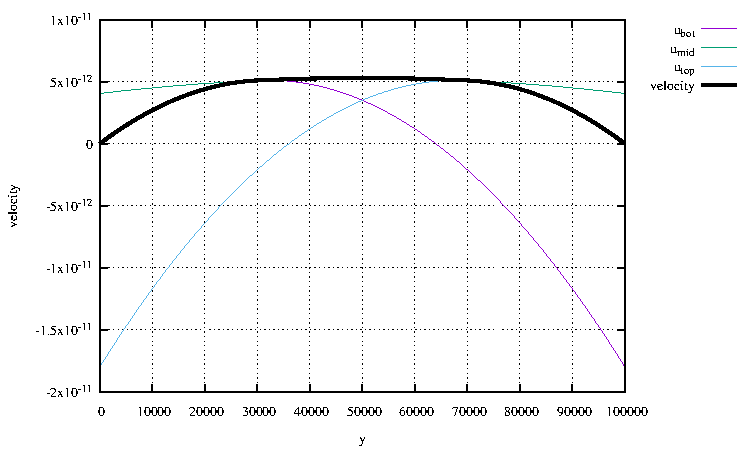
\includegraphics[width=7cm]{images/mms/channel_hb/velocity}
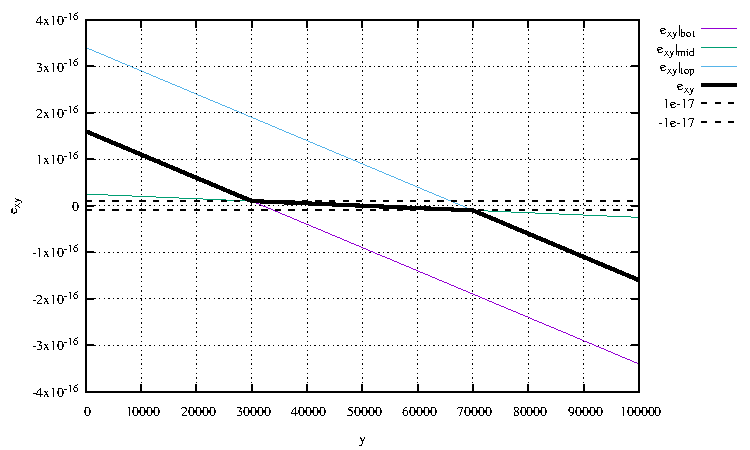
\includegraphics[width=7cm]{images/mms/channel_hb/exy}\\
{\captionfont Obtained for $n=1$ and $\tau_0=9e7$. The black lines are the resulting velocity and strain rate profiles obtained by joining the bottom, middle and top functions.}
\end{center}

In the following I explore the effect of the $\tau_0$ value ($K$ is calculated correspondingly as we have seen before).

\begin{center}
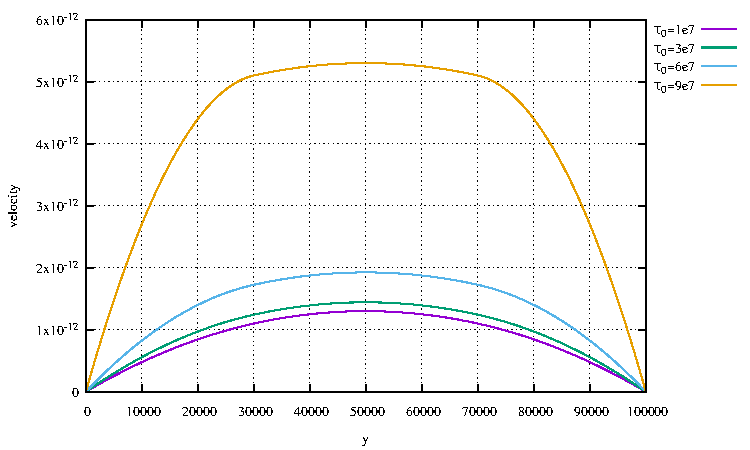
\includegraphics[width=7.5cm]{images/mms/channel_hb/velocity_taus}
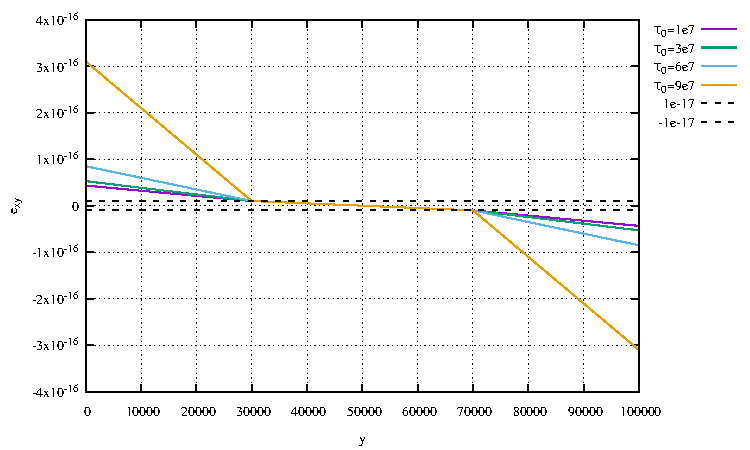
\includegraphics[width=7.5cm]{images/mms/channel_hb/exy_taus}\\
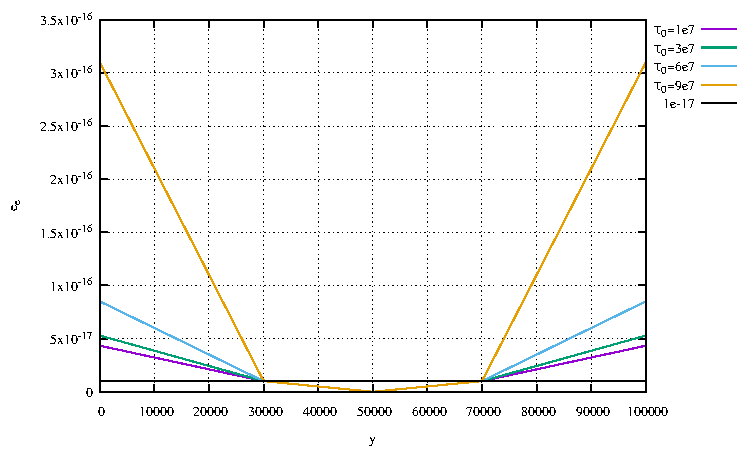
\includegraphics[width=7.5cm]{images/mms/channel_hb/ee_taus}
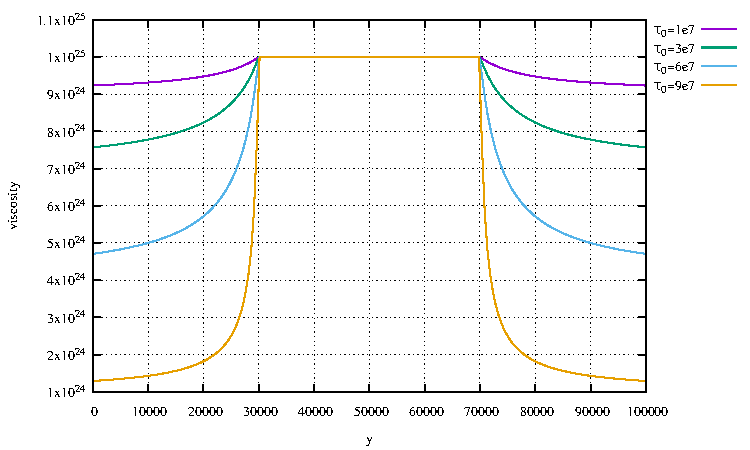
\includegraphics[width=7.5cm]{images/mms/channel_hb/eta_taus}
\end{center}






\newpage
%-----------------------------------------------------------------------------
\subsubsection{Flow in a square using Stream Functions \label{ss:square_streamfct} }

I wish to arrive at an analytical formulation for a 2D incompressible flow in the square domain $[-1:1]\times[-1:1]$
The fluid has constant viscosity $\eta=1$ and is subject to free slip boundary conditions on all sides.
For reasons that will become clear in what follows I postulate the following stream function:
\begin{equation}
\Psi(x,y)=\sin( m \pi x)\sin( n\pi y)
\end{equation}
We have the velocity being defined as:
\begin{mdframed}[backgroundcolor=blue!5]
\begin{equation}
{\vec \upnu} = (u,v) = \left( \frac{\partial \Psi}{\partial y},-\frac{\partial \Psi}{\partial x} \right) 
= (n \pi \sin (m\pi x)\cos(n\pi y),-m\pi \cos(m\pi x)\sin (n\pi y))
\end{equation}
\end{mdframed}

\begin{center}
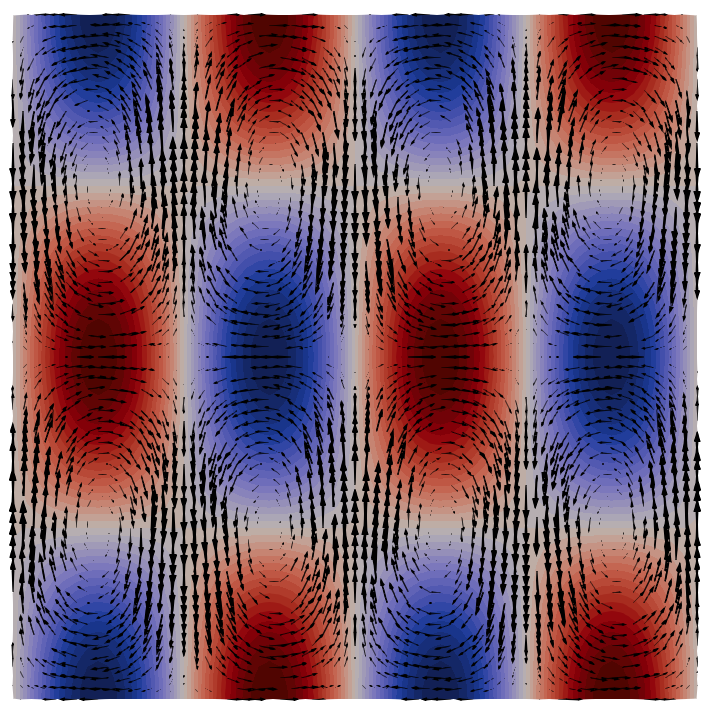
\includegraphics[width=5cm]{images/mms/square_streamfunction/vel_2x1}\\
{\captionfont Velocity field for $(m,n)=(2,1)$}
\end{center}

The strain rate components are then:
\begin{eqnarray}
\dot\varepsilon_{xx} &=&  \frac{\partial u}{\partial x} = mn \pi^ 2  \cos (m\pi x)\cos(n\pi y)   \\
\dot\varepsilon_{yy} &=&  \frac{\partial v}{\partial y} = -mn \pi^ 2  \cos (m\pi x)\cos(n\pi y)  \\
2\dot\varepsilon_{xy} &=&  \frac{\partial u}{\partial y} +  \frac{\partial v}{\partial x}    \\
&=&  \frac{\partial^2 \Psi}{\partial y^2} -  \frac{\partial^2 \Psi}{\partial x^2}    \\
&=& -n^2\pi^2 \Psi + m^2 \pi^2 \Psi \\
&=& (m^2-n^2) \pi^2   \sin( m \pi x)\sin( n\pi y)
\end{eqnarray}
Note that if $m=n$ the last term is identically zero, which is not desirable 
(flow is too 'simple')
so in what follows we will prefer $m\neq n$.

It is also easy to verify that $u=0$ on the sides and $v=0$ at the top and bottom and that the 
term $\dot\varepsilon_{xy}$ is nul on all four sides, thereby garanteeing free slip. 

Our choice of stream function yields:
\[
{\nabla}^4 \Psi= 
\frac{\partial^4 \Psi}{\partial x^4}+
\frac{\partial^4 \Psi}{\partial y^4}+
2\frac{\partial^2 \Psi}{\partial x^2 y^2}
=\pi^4 ( m^4 \Psi + n^4 \Psi + 2m^2n^2 \Psi) = (m^4 + n^4 + 2m^2n^2)\pi^4 \Psi
\]

Let us recall Eq.~(\ref{eq:sf1}):
\begin{equation}
{\vec \nabla}^4 \Psi 
=
-\frac{\partial \rho g_y}{\partial x} + \frac{\partial \rho g_x}{\partial y}   
\end{equation}
We assume $g_x=0$ and $g_y=-1$ so that we simply have 
\begin{equation}
\frac{\partial \rho}{\partial x}
=
(m^4 + n^4 + 2m^2n^2)\pi^4 \Psi 
=
(m^4 + n^4 + 2m^2n^2)\pi^4 \sin( m \pi x)\sin( n\pi y)
\end{equation}
so that (assuming the integration constant to be zero):
\[
\rho(x,y) = -\frac{m^4 + n^4 + 2m^2n^2}{m} \pi^3  \cos(m \pi x)\sin(n \pi y)
\]
The $x$-component of the momentum equation is (since $g_x=0$): 
\[
-\frac{\partial p}{\partial x} + 
\frac{\partial^2 u}{\partial x^2}+
\frac{\partial^2 u}{\partial y^2} =
-\frac{\partial p}{\partial x} 
-m^2 n \pi^3 \sin (m\pi x)\cos(n\pi y)
- n^3 \pi^3 \sin (m\pi x)\cos(n\pi y)
=0
\]
so 
\[
\frac{\partial p}{\partial x} =-(m^2n+n^3)\pi^3 \sin (m\pi x)\cos(n \pi y)
\]
and the pressure field is then (once again neglecting the integration constant):
\begin{mdframed}[backgroundcolor=blue!5]
\[
p(x,y)= \frac{m^2n+n^3}{m} \pi^2 \cos (\pi x)\cos(\pi y)
\]
\end{mdframed}
Note that we then have the interesting property that the pressure average 
over the domain is zero, i.e. $\int p dV =0$.





%-------------------------------------------------------------------------------
\subsubsection{One-dimensional advection-diffusion equation \label{ss:advdiff} }

Let us start with the 1D steady advection-diffusion equation:
\begin{equation}
\rho C_p u \frac{dT}{dx} - k \frac{d^2T}{dx^2} = f \qquad \text{in} \quad [0,L_x]
\end{equation}
with the boundary conditions $T(x=0)=0$ and $T(x=L_x)=0$.

The solution to this problem is:
\[
T(x) = \frac{f}{u}\left( x - \frac{1-\exp \frac{ux}{\kappa}}{1-\exp \frac{u}{\kappa} } \right)
\]
or 
\[
T(x) = \frac{f}{u}\left( x - \frac{1-\exp \frac{2 Pe x}{h}}{1-\exp \frac{2 Pe}{h} } \right)
\]
where
\[
Pe = \frac{uh}{2 \kappa} = \frac{u h \rho C_p}{2 k}
\]


%..............................................................................
\subsubsection{Annulus with kinematical b.c. - shear flow}\label{ss:sfan}

Let us consider an annulus domain of inner radius $R_1$ and outer radius $R_2$.
Boundary conditions are $\vec\upnu(r=R_1)=\upnu_1 \vec{e}_\theta$ and 
$\vec\upnu(r=R_2)=\upnu_2 \vec{e}_\theta$. Density is assumed to be zero in the domain. 

As seen in Section~\ref{ss:ankbc}, the Laplacian of a vector $\vec{A}$ is given 
by\footnote{\url{https://en.wikipedia.org/wiki/Vector\_Laplacian}} 
\[
\nabla^2 \vec{A} = \nabla(\nabla\cdot\vec{A}) - \nabla\times(\nabla \times\vec{A})
=
\left(
\begin{array}{l}
\frac{\partial^2 A_r}{\partial r^2} + \frac{1}{r} \frac{\partial A_r}{\partial r} - \frac{1}{r^2} A_r  + \frac{1}{r^2} \frac{\partial^2 A_r}{\partial \theta^2}  - \frac{2}{r^2} \frac{\partial A_\theta}{\partial \theta} \\ \\
\frac{\partial^2 A_\theta}{\partial r^2} + \frac{1}{r} \frac{\partial A_\theta}{\partial r} - \frac{1}{r^2} A_\theta  + \frac{1}{r^2} \frac{\partial^2 A_\theta}{\partial \theta^2}  + \frac{2}{r^2} \frac{\partial A_r}{\partial \theta} 
\end{array}
\right)
\]
%=
%\left(
%\begin{array}{l}
%\Delta A_r \\ \\ \Delta A_\theta
%\end{array}
%\right)
Given the symmetry of the problem and the boundary conditions we know that the 
solution is as follows: 
\[
{\vec \upnu}(r,\theta) = \upnu_\theta(r) {\vec e}_\theta
\]

Using this velocity field, we can now obtain the pressure field 
by solving the Stokes equation
\[
-\vec\nabla p + \eta {\vec\nabla}^2 {\vec \upnu} = {\vec 0}
\]
since density is zero. Because of symmetry we also expect the pressure to
be a function of $r$ only, i.e. $p(r)$.
The Stokes equation in polar coordinates then writes:
\begin{eqnarray}
-\frac{\partial p}{\partial r} &=& 0 \\
-\frac{1}{r}\underbrace{\frac{\partial p}{\partial \theta}}_{=0} + 
\frac{\partial^2 \upnu_\theta}{\partial r^2} + \frac{1}{r} \frac{\partial \upnu_\theta}{\partial r} 
- \frac{1}{r^2} \upnu_\theta  &=&0 
\end{eqnarray}
so that the pressure is a constant which we arbitrarily set to zero. 
We assume $\upnu_\theta(r) = r^\alpha$, and the second equation above becomes: 
\[
\alpha(\alpha-1) r^{\alpha-2}  + \alpha r^{\alpha-2}  - r^{\alpha-2}  = 0 
\]
reducing to $\alpha^2-1=0$, i.e. $\alpha=\pm 1$, since the above equation must be valid
for any value of $r$.
The generic solution then can be written as
\[
\upnu_\theta (r) = A r + \frac{B}{r}
\]
Using the b.c. : 
\[
\upnu_\theta (R_1) = A R_1 + \frac{B}{R_1} = \upnu_1
\]
\[
\upnu_\theta (R_2) = A R_2 + \frac{B}{R_2} = \upnu_2
\]
or, 
\[
A + \frac{B}{R_1^2} = \frac{\upnu_1}{R_1}
\]
\[
A + \frac{B}{R_2^2} = \frac{\upnu_2}{R_2}
\]
so
\[
B=\frac{ \frac{\upnu_1}{R_1}-\frac{\upnu_2}{R_2}  }{\frac{1}{R_1^2} - \frac{1}{R_2^2}} = 
R_1R_2 \frac{ \upnu_1R_2-\upnu_2R_1    }{R_2^2-R_1^2}
\]
and 
\[
A=\frac{\upnu_2R_2-\upnu_1R_1}{R_2^2-R_1^2}
\]
%\includegraphics[width=10cm]{PROJECTS/annulus/velprof}

We can verify that the flow is indeed incompressible:
\[
\vec\nabla\cdot\vec\upnu = \frac{1}{r}\frac{\partial (r\upnu_r)}{\partial r} 
+ \frac{1}{r}\frac{\partial \upnu_\theta}{\partial \theta} = 0
\]
since $\upnu_r=0$ and $\upnu_\theta$ does not depend on $\theta$.

Note that we could have used a non-zero density: as long as it does not 
depend on $\theta$ and the gravity points towards the center,
it allows for a decoupling of the equations, thereby 
only contributing to a lithostatic pressure field.

%..............................................................................
\subsubsection{Generic framework for 3D solution in Cartesian coordinates}\label{ss:mms3Dgen}

We postulate
\begin{eqnarray}
u(x,y,z) &=& f(x) g'(y) h'(z) \\
v(x,y,z) &=& f'(x) g(y) h'(z) \\
w(x,y,z) &=& -2f'(x) g'(y) h(z) 
\end{eqnarray}
so that the flow is indeed incompressible: 
\[
\frac{\partial u}{\partial x}+
\frac{\partial v}{\partial y}+
\frac{\partial w}{\partial z}
=
f'(x) g'(y) h'(z) + f'(x) g'(y) h'(z) -2f'(x) g'(y) h'(z)
=0
\]
The velocity gradient ${\bm L}(\vec\upnu)$ is then given by
\[
{\bm L}(\vec\upnu) =
\left(
\begin{array}{ccc}
f'g'h' &  f'' g h' & -2f'' g' h \\ \\
fg''h' & f'g'h'    & -2f' g'' h \\ \\
fg'h'' & f'gh''    & -2f'g'h'
\end{array}
\right)
\]
and the strain rate tensor by:
\[
\dot{\bm \varepsilon}(\vec\upnu)
=\frac{1}{2}({\bm L}(\vec\upnu)+{\bm L}(\vec\upnu)^T)
=
\frac{1}{2}
\left(
\begin{array}{ccc}
2f'g'h' & (f'' g+fg'') h'  & fg'h''-2f'' g' h \\ \\
(f''g+fg'')h' & 2f'g'h'    & f'gh''-2f' g'' h \\ \\
fg'h'' -2f'' g' h & f'gh'' -2f' g'' h    & -4f'g'h'
\end{array}
\right)
\]

We assume for simplicity that $\eta=1$ so 
\begin{eqnarray}
\vec\nabla\cdot 2\eta \dot{\bm \varepsilon}(\vec\upnu)
&=&
\vec\nabla\cdot \left(
\begin{array}{ccc}
2f'g'h'           & (f'' g+fg'') h'    & fg'h''-2f'' g' h \\ \\
(f''g+fg'')h'     & 2f'g'h'            & f'gh''-2f' g'' h \\ \\
fg'h'' -2f'' g' h & f'gh'' -2f' g'' h  & -4f'g'h'
\end{array}
\right) \nn\\
&=&
\left(
\begin{array}{c}
2f''g'h' +    (f''g'+fg''')h'   +   fg'h''' -2f'' g' h'   \\ \\
(f''' g+f'g'') h'  +     2f'g''h'   +     f'gh''' -2f' g'' h' \\ \\
f'g'h''-2f''' g' h   +  f'g'h''-2f' g''' h     -4f'g'h''
\end{array}
\right) \nn\\
&=&
\left(
\begin{array}{c}
f''g' h'  + fg''' h'  +  fg'h'''   \\ \\
f''' g h' + f'g'' h'  +  f'gh'''  \\ \\
-2f''' g' h     -2f' g''' h -2f'g'h''
\end{array}
\right) 
\end{eqnarray}
The Stokes equation then writes 
\[
\left(
\begin{array}{c}
-\partial_x p \\ \\
-\partial_y p \\ \\
-\partial_z p 
\end{array}
\right) 
+
\left(
\begin{array}{c}
f''g' h'  + fg''' h'  +  fg'h'''   \\ \\
f''' g h' + f'g'' h'  +  f'gh'''  \\ \\
-2f''' g' h     -2f' g''' h -2f'g'h''
\end{array}
\right) 
+
\left(
\begin{array}{c}
b_x \\ \\ b_y \\ \\ b_z
\end{array}
\right) 
=\vec{0}
\]
or, 
\[
\left(
\begin{array}{c}
b_x \\ \\ b_y \\ \\ b_z
\end{array}
\right) 
=
\left(
\begin{array}{c}
\partial_x p \\ \\
\partial_y p \\ \\
\partial_z p 
\end{array}
\right) 
-
\left(
\begin{array}{c}
f''g' h'  + fg''' h'  +  fg'h'''   \\ \\
f''' g h' + f'g'' h'  +  f'gh'''  \\ \\
-2f''' g' h     -2f' g''' h -2f'g'h''
\end{array}
\right) 
\]

%..............................
\paragraph{First application}


Let us assume 
\[
f(x)=x(1-x) \qquad
g(y)=y(1-y) \qquad
h(z)=z(1-z) 
\]
then 
\[
f'(x)=1-2x \qquad
g'(y)=1-2y \qquad
h'(z)=1-2z 
\]
\[
f''(x)=-2 \qquad
g''(y)=-2 \qquad
h''(z)=-2 
\]
\[
f'''(x)=0 \qquad
g'''(y)=0 \qquad
h'''(z)=0 
\]
Which ensures that there is no flow through the boundaries of the unit cube.
Then 
\[
\left(
\begin{array}{c}
b_x \\ \\ b_y \\ \\ b_z
\end{array}
\right) 
=
\left(
\begin{array}{c}
\partial_x p \\ \\
\partial_y p \\ \\
\partial_z p 
\end{array}
\right) 
-
\left(
\begin{array}{c}
f''g' h'     \\ \\
f'g'' h'    \\ \\
-2f'g'h''
\end{array}
\right) 
\]
with 
\begin{eqnarray}
u(x,y,z) &=& x(1-x)(1-2y)(1-2z)\\
v(x,y,z) &=& (1-2x) y(1-y) (1-2z) \\
w(x,y,z) &=& -2(1-2x)(1-2y)z(1-z)
\end{eqnarray}

Finally we postulate 
\[
p(x,y,z) = (2x-1)(2y-1)(2z-1)
\]
with $\int_\Omega p(x,y,z) dx dy dz =0$, so
\[ 
\left(
\begin{array}{c}
\partial_x p \\ \\
\partial_y p \\ \\
\partial_z p 
\end{array}
\right) 
=
\left(
\begin{array}{c}
2(2y-1)(2z-1) \\\\
2(2x-1)(2z-1) \\\\
2(2x-1)(2y-1) 
\end{array}
\right) 
\]
Then we find that 
\[
\vec{b}
=
\left(
\begin{array}{c}
2(2y-1)(2z-1) -(-2)(1-2y)(1-2z) \\
2(2x-1)(2z-1) -(1-2x)(-2)(1-2z) \\
2(2x-1)(2y-1) +2(1-2x)(1-2y)(-2)
\end{array}
\right)
=
\left(
\begin{array}{c}
4(2y-1)(2z-1)\\ \\
4(2x-1)(2z-1) \\ \\
-2(2x-1)(2y-1) 
\end{array}
\right)
\]


The root mean square velocity is given by 
\begin{eqnarray}
\int_\Omega u^2 dV &=& 1/270 \\
\int_\Omega v^2 dV &=& 1/270 \\
\int_\Omega w^2 dV &=& 2/135
\end{eqnarray}
and then 
\[
\upnu_{vrms} =\sqrt{\frac{6}{270}} \simeq 0.1490712
\]

This benchmark is implemented in \stone 10 ($Q_1\times P_0$), 
%\stone 75 (MINI-1 bubble) 
and \stone 82 (MINI-2 bubbles).  
The code is available in {\tt /mms/mms3D.py}.

\begin{center}
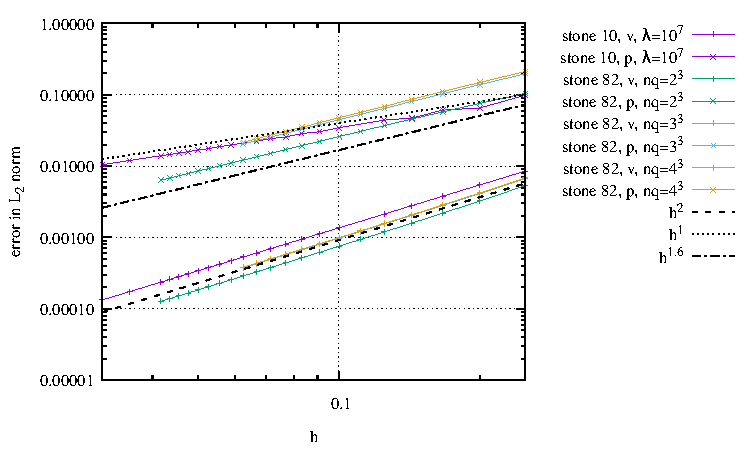
\includegraphics[width=7cm]{images/mms/generic3D/conv.pdf}
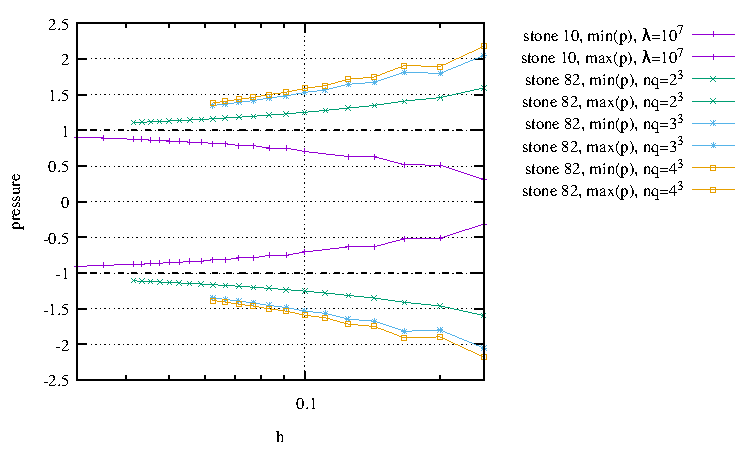
\includegraphics[width=7cm]{images/mms/generic3D/p_stats.pdf}\\
{\captionfont Error convergence and pressure statistics}
\end{center}

%..................................
\paragraph{Second application}

Once again, no flow through the boundaries of the unit cube:
\[
f(x)=x^2(1-x)^2 \qquad
g(y)=y^2(1-y)^2 \qquad
h(z)=z^2(1-z)^2 
\]
then 
\[
f'(x)=2x(2x^2-3x+1) \qquad
g'(y)=2y(2y^2-3y+1) \qquad
h'(z)=2z(2z^2-3z+1) 
\]
\[
f''(x)=2(6x^2-6x+1) \qquad
g''(y)=2(6y^2-6y+1) \qquad
h''(z)=2(6z^2-6z+1)
\]
\[
f'''(x)=24x-12 \qquad
g'''(y)=24y-12 \qquad
h'''(z)=24z-12
\]
The velocity field is then given by
\begin{eqnarray}
u(x,y,z) 
&=& f(x) g'(y) h'(z) 
= 4 x^2(1-x)^2  y(2y^2-3y+1) z(2z^2-3z+1)  \nn\\
v(x,y,z) 
&=& f'(x) g(y) h'(z) 
= 4 x(2x^2-3x+1) y^2(1-y)^2 z(2z^2-3z+1) \nn\\
w(x,y,z) 
&=& -2f'(x) g'(y) h(z) 
= -8 x(2x^2-3x+1) y(2y^2-3y+1) z^2(1-z)^2 
\end{eqnarray}
We choose
\[
p(x,y,z)=f'g'h' = 2x(2x^2-3x+1)  2y(2y^2-3y+1)  2z(2z^2-3z+1) 
\]













%..........................................................
\subsubsection{2D Analytical benchmark XII}\label{ss:sofo87_2D}

This is presented in Soulaimani et al (1987) \cite{sofo87}. 
The velocity field is given by
\[
\vec\upnu(x,y) = (x^3,-3x^2y) 
\]
and the pressure is 
\[
p(x,y)=x^3+y^3-1/2
\]
so that, assuming that the viscosity is 1, the body force is:
\[
\vec{b} = (-6x+3x^2,6y+3y^2)
\] 
Note that I have added the $-1/2$ term to the pressure so that $\int\int p dxdy=0$.
The root mean square velocity over a unit square is 
\[
\upnu_{rms} 
= \sqrt{ \int_0^1\int_0^1 (u^2+v^2) dx dy }
= \sqrt{ \int_0^1\int_0^1 (x^6 + 9 x^4 y^2) dx dy }
= \sqrt{ \frac{1}{7} + 9 \frac{1}{5} \frac{1}{3}  } 
= \sqrt{ \frac{26}{35} }
\simeq 0.861892 
\]
The strain rate tensor terms are
\begin{eqnarray}
\dot{\varepsilon}_{xx} &=& 3x^2  \nonumber\\
\dot{\varepsilon}_{yy} &=& -3x^2 \nonumber\\ 
\dot{\varepsilon}_{xy} &=& -3xy  \nn
\end{eqnarray}

Another one mentioned in the paper:
\[
\vec\upnu(x,y) =(x^2,-2xy)
\qquad
p(x,y)=0
\qquad
\vec{b}=(-2,0) 
\]

%..........................................................
\subsubsection{2D Analytical benchmark XIII}\label{ss:sofo87_3D}

This is presented in Soulaimani et al (1987) \cite{sofo87}. 

\[
\vec{b} = (1,1,1)
\qquad
\vec{\upnu}(x,y,z)=(y,z,x)
\qquad
p(x,y,z)=x+y+z-1/2
\]


%..........................................................
\subsubsection{Poisson equation on 3D shell} 

This benchmark is presented in Phillips \etal \cite{phdo19}. 
Inner radius is 1, outer radius is 3.
The right hand side term of the Poisson equation is given by:
\begin{eqnarray}
f(r,\theta,\phi)&=&
\frac{\sin^2\theta }{R^2} 
\left[
(\cos\phi-\sin\phi)(20\sin^2\theta -15) -\sin 2\phi (10\sin^2 \theta -6)
\right] \nn\\
&\times & \left[ \left(\frac{r}{R_{inner}}\right)^2 -1  \right]
\left[ \left(\frac{r}{R_{outer}}\right)^2 -1  \right] \nn\\
&+&\sin^4 \theta
\left[ \cos\phi -\sin\phi -\frac12 \sin 2\phi \right]
\left[
\frac{20r^2}{R_{inner}^2R_{outer}^2} -6 \left( \frac{1}{R_{inner}^2}+\frac{1}{R_{outer}^2}  \right)
\right]
\end{eqnarray}
Note: what is $R$ here??

The solution is then 
\[
T(r,\theta,\phi) = \sin^4 \theta \left[ \cos\phi -\sin\phi -\frac12 \sin 2\phi \right]
\left[ \left(\frac{r}{R_{inner}}\right)^2 -1  \right]
\left[ \left(\frac{r}{R_{outer}}\right)^2 -1  \right]
\]
This expression is used to generate the Dirichlet boundary conditions on the inner and outer surfaces.


%..........................................................
\subsubsection{SolCx}\label{ss:solcx} 

%Taken from aspect manual. 
The SolCx benchmark is intended to test the accuracy of the solution to a problem that 
has a large jump in the viscosity along a line through the domain. Such situations are 
common in geophysics: for example, the viscosity in a cold, subducting slab is much larger 
than in the surrounding, relatively hot mantle material.

The SolCx benchmark computes the Stokes flow field of a fluid driven by spatial density 
variations, subject to a spatially variable viscosity. Specifically, the domain 
is $\Omega = [0,1]^2$, gravity is $\vec{g} = (0,-1)^T$ and the density is given by 
\begin{equation}
\rho(x,y) = \sin(\pi y) \cos(\pi x)
\end{equation}
Boundary conditions are free slip on all of the sides of the domain and the 
temperature plays no role in this benchmark. 
The viscosity is prescribed as follows:
\begin{equation}
\eta(x,y) = 
\left\{
\begin{array}{lll}
1 & \text{for} & x<0.5 \\
10^6 & \text{for} & x>0.5 \\
\end{array}
\right.
\end{equation}
Note the strongly discontinuous viscosity field yields a stagnant flow 
in the right half of the domain and thereby yields a pressure discontinuity along the interface. 

The SolCx benchmark was previously showcased in Duretz \etal (2011) \cite{dumg11} 
and its analytic solution is given in Zhong (1996) \cite{zhon96}. 
It has been carried out in Kronbichler \etal (2012) \cite{krhb12} and Gerya \etal (2013) \cite{gemd13}, 
and is also found in the \aspect manual \cite{aspectmanual}. 

Note that the source code which evaluates the velocity and pressure fields for both SolCx and SolKz is 
distributed as part of the open source package Underworld 
(Moresi \etal, 2007 \cite{moql07}, http://underworldproject.org).
I have translated this code to python. 

\begin{center}
a)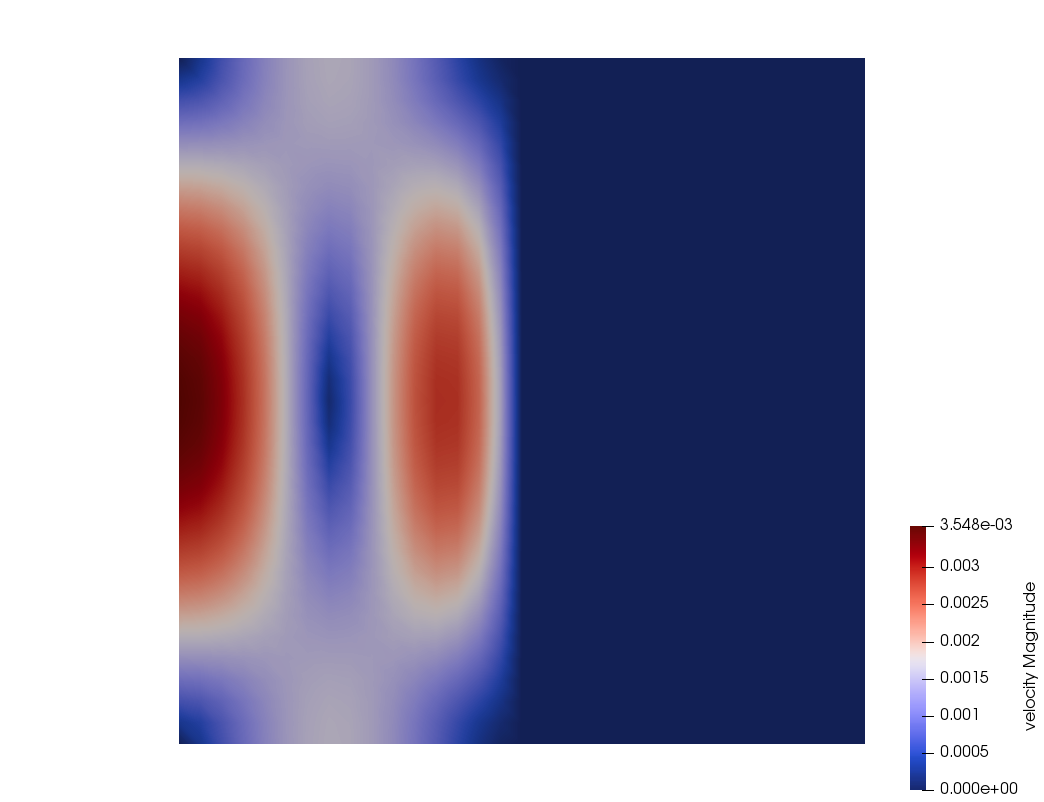
\includegraphics[width=5cm]{images/benchmark_solcx/vel}
b)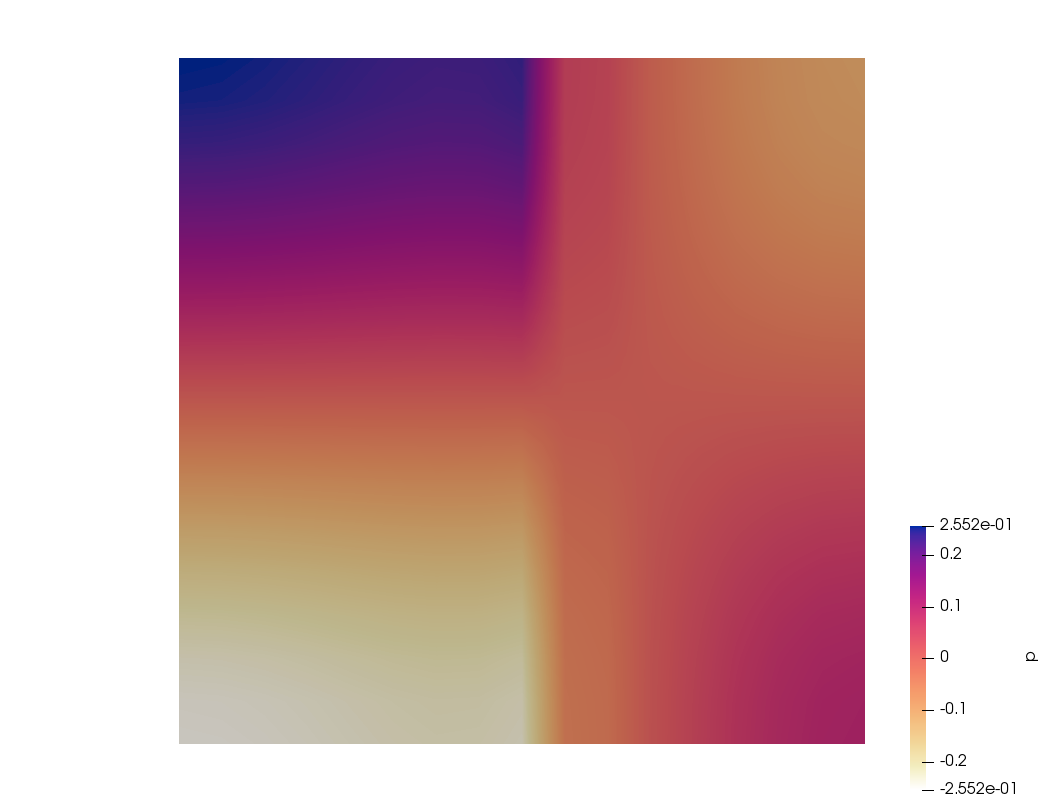
\includegraphics[width=5cm]{images/benchmark_solcx/press}\\
c)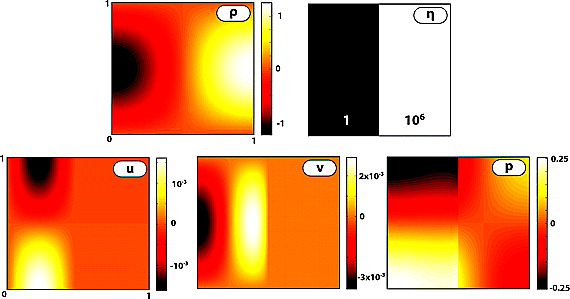
\includegraphics[width=10cm]{images/benchmark_solcx/dumg11}\\
{\captionfont a,b) obtained with \aspect. c) taken from Duretz \etal (2011) \cite{dumg11}.}
\end{center}

\begin{center}
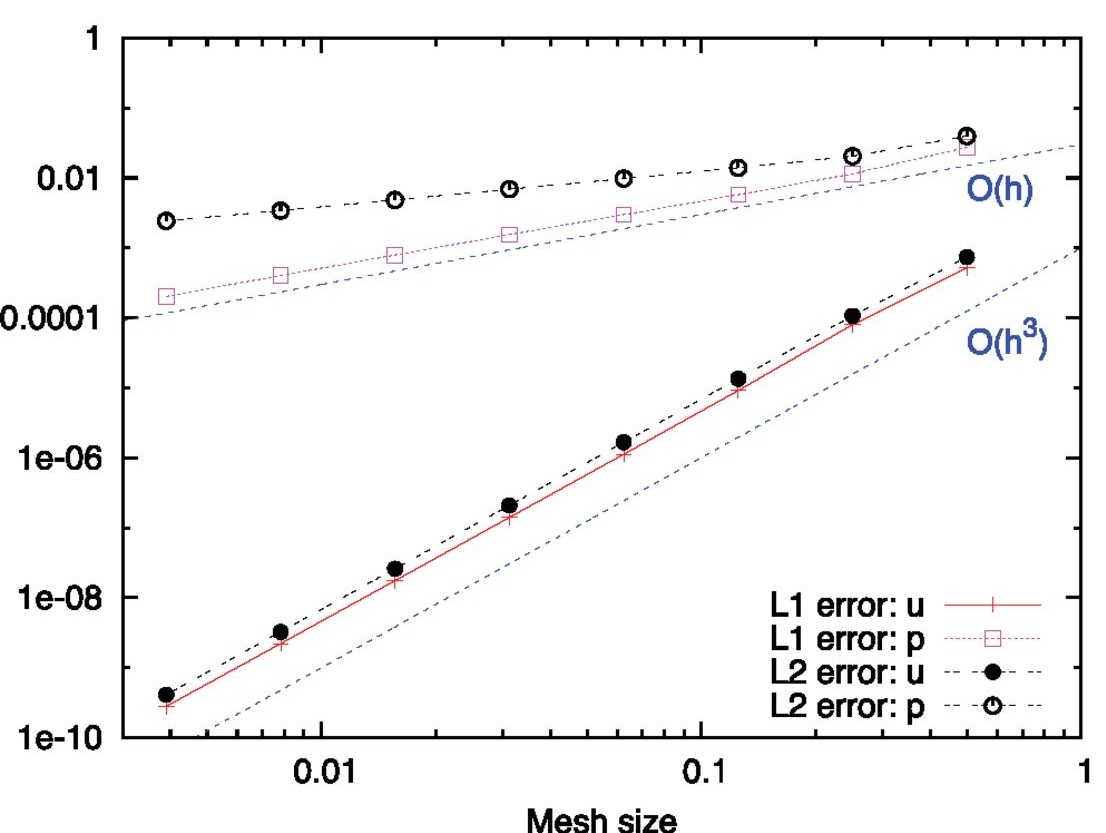
\includegraphics[width=5cm]{images/benchmark_solcx/krhb12}
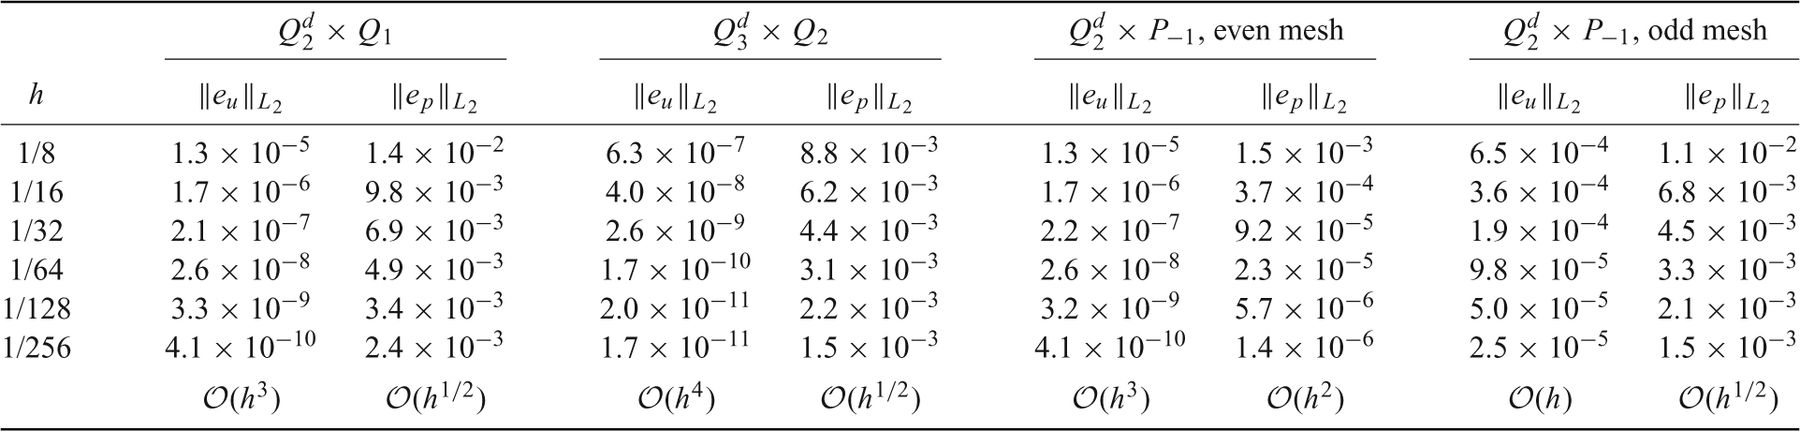
\includegraphics[width=11cm]{images/benchmark_solcx/krhb12b}\\
{\captionfont Taken from Kronbichler \etal (2012) \cite{krhb12}.
Velocity and pressure errors eu, ep and convergence rates for different choices of 
the Stokes finite element spaces, using globally refined meshes. 
For `odd' meshes, the numbers shown are the average errors from nearby meshes 
(e.g. for $h=1/64$, the average of the errors on 63x63 and 65x65 meshes).}
\end{center}


\Literature: \cite{mamo08,vemmXX,demh19} 

\stones 5, 77





%..........................................................
\subsubsection{SolKz} \label{ss:solkz} 


The SolKz benchmark is similar to the SolCx benchmark: 
the viscosity is a function of the space coordinates too and is given by 
\[
\eta(y)=\exp(2By) \quad {\rm with} \quad B=13.8155
\]
It is not a discontinuous function but grows exponentially with the 
vertical coordinate so that its overall variation is again $10^6$. 
The forcing is again chosen by imposing a spatially variable density variation as follows:
\[
\rho(x,y)=\sin(2y) \cos(3\pi y)
\]
Free slip boundary conditions are imposed on all sides of the domain.
This benchmark too is presented in \cite{zhon96} and is studied in \cite{dumg11} and \cite{gemd13}.

\begin{center}
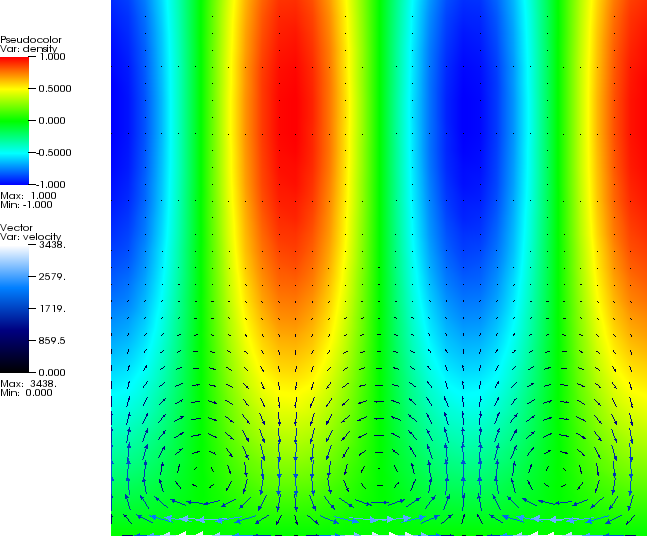
\includegraphics[width=6cm]{images/benchmark_solkz/solkz-solution}
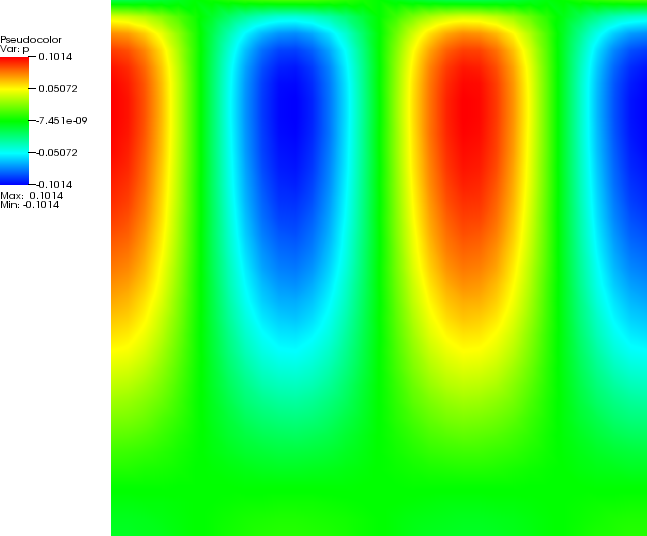
\includegraphics[width=6cm]{images/benchmark_solkz/solkz-solution-pressure}\\
{\captionfont Taken from \aspect manual \cite{aspectmanual}.}
\end{center}


\begin{center}
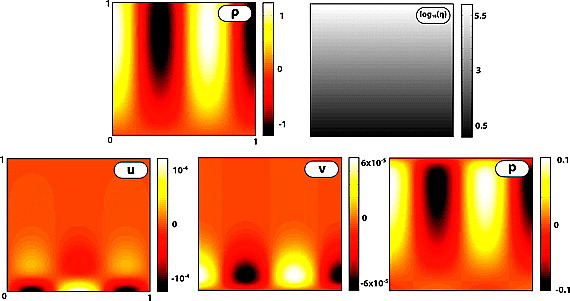
\includegraphics[width=10cm]{images/benchmark_solkz/dumg11}\\
{\captionfont Taken from Duretz \etal (2011) \cite{dumg11}.}
\end{center}

\Literature: \cite{mozg96}, \cite{mamo08}, \cite{vemmXX}, \cite{demh19}, \cite{repa87}
\stone 06


%..........................................................
\subsubsection{SolVi} \label{ss:solvi} 
SolVi is another very common benchmark carried out in the computational 
geodynamics literature.

This inclusion benchmark solves a problem with a discontinuous viscosity, 
which is chosen in such a way that the discontinuity is a circle. 
Given the regular nature of the used by a majority of codes, 
this ensures that the discontinuity in the viscosity never aligns to cell boundaries.
This in turns leads to almost discontinuous pressures along the interface which are difficult 
to represent accurately.

Schmid \& Podlachikov (2003) \cite{scpo03}. 
derived a simple analytic solution for the pressure and velocity fields for such a circular 
inclusion under simple shear.

A characteristic of the analytical solution is that the pressure is zero 
inside the inclusion, while outside it follows the relation
\[
p_m = 4 \dot{\epsilon}
\frac{\eta_m(\eta_i-\eta_m)}{\eta_i+\eta_m}
\frac{r_i^2}{r^2} \cos(2\theta)
\]
where $\eta_i$ is the viscosity of the inclusion (often taken to be 1000)
and $\eta_m1$ is the viscosity of the background media (often taken to be 1). 

One important observation with this benchmark is the fact that the velocity is not zero even far 
away from the inclusion, so that the analytical solution must be imposed on the sides.
Also, because of symmetry, it is often run on the top quadrant $x>0$, $y>0$ with 
free slip imposed on the left and bottom boundaries. 

\begin{center}
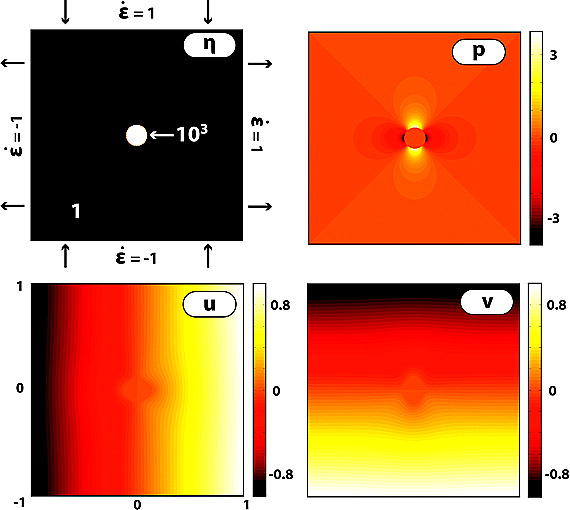
\includegraphics[width=9cm]{images/benchmark_solvi/dumg11}
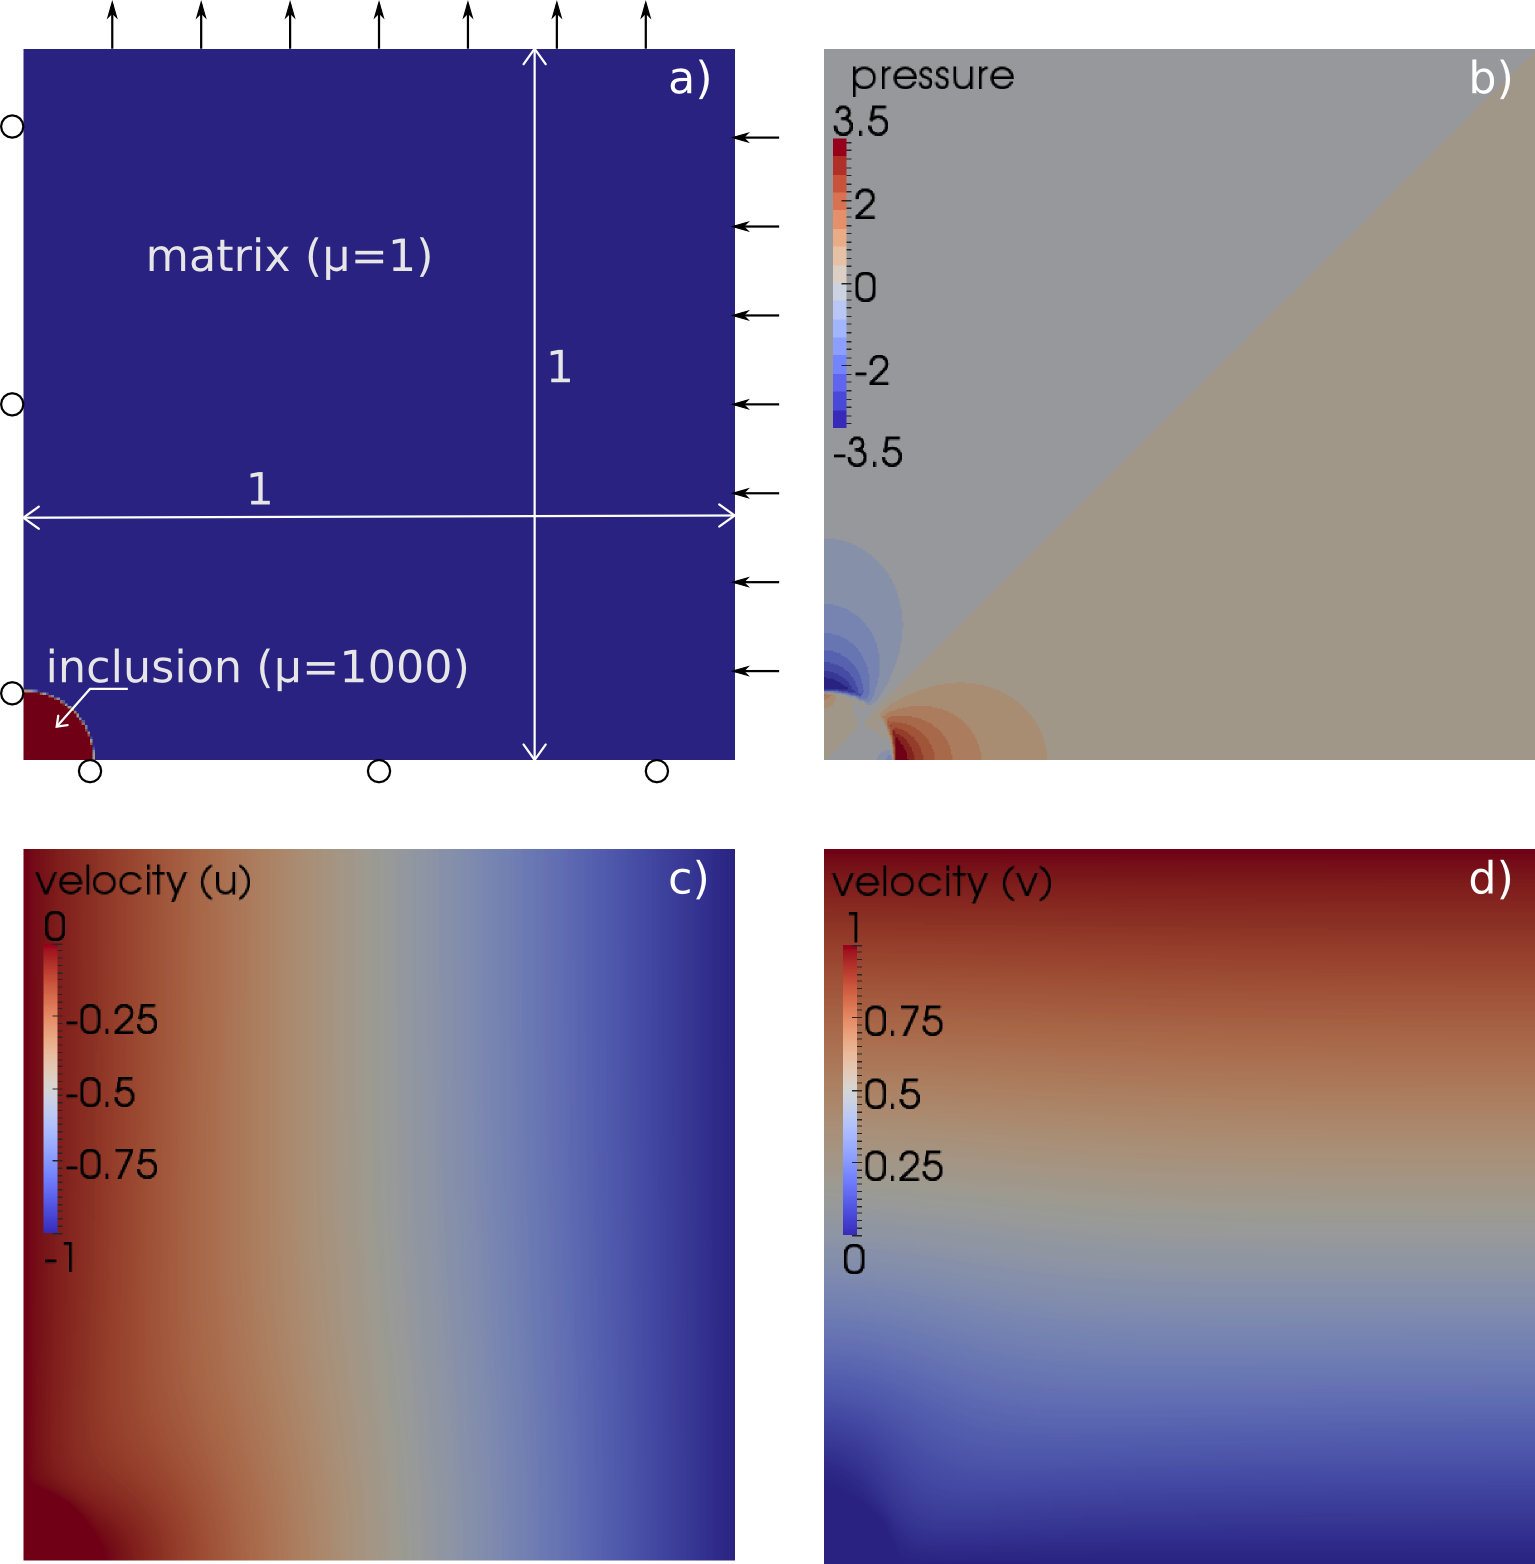
\includegraphics[width=7cm]{images/benchmark_solvi/drawing}\\
{\captionfont Left: taken from Duretz \etal (2011) \cite{dumg11}. }
\end{center}

\Literature: 
\textcite{kapo06},
\textcite{maie12},
\textcite{deka08},
\textcite{bepo10},
\textcite{sunh10},
\textcite{vosc15},
\textcite{demh19},
\textcite{aspectmanual},
\textcite{litu02},
\stone~07,
\textcite{krhb12}, 
\textcite{gemd13}.













